\documentclass[english, LaM, oneside, noexaminfo]{sapthesis}
\usepackage[utf8]{inputenx}
\usepackage{indentfirst}
\usepackage{microtype}
\usepackage[nottoc, notlof, notlot]{tocbibind}
%\onehalfspacing
%\counterwithout{footnote}{chapter}
\usepackage{hyperref}

\usepackage{amsfonts}
\usepackage{amssymb}
\usepackage{amsthm}
\usepackage{amsmath}
\usepackage{nicefrac}
\usepackage{tocbibind}
\usepackage[T1]{fontenc}
\usepackage{ytableau}
\usepackage{mathdots}
\usepackage{mathabx}
\usepackage{subfigure}
\usepackage{booktabs}
\usepackage{makecell}
\usepackage{tabularx}
\usepackage{pdfpages}


\usepackage[
backend=biber,
style=alphabetic,
sorting=ynt
]{biblatex}

\usepackage[center]{subfigure}



\newtheorem{teo}{\bf Theorem}[section]
\newtheorem{prop}{\bf Proposition}[section]
\newtheorem{lem}{\bf Lemma}[section]
\newtheorem{oss}{\bf Remark}[section]
\newtheorem{defin}{\bf Definition}[section]
\newtheorem{cor}{\bf Corollary}[section]
\newtheorem{es}{\bf Example}[section]
\newtheorem{notaz}{\bf Notation}[section]

\addbibresource{bibliography.bib}

\title{Bridging Topological Persistence and Machine Learning for Music Information Retrieval}
\author{Luca Sassone}
\IDnumber{1544447}
\course{Matematica}
\courseorganizer{Facoltà di Scienze Matematiche Fisiche e Naturali}
\copyyear{2021}
\AcademicYear{2020/2021}
\advisor{Prof. Marco Manetti}
\coadvisor{Prof. Massimo Ferri}
\coadvisor{Dr. Mattia G. Bergomi}
\authoremail{sassone.1544447@studenti.uniroma1.it}



%we refer to http://ctan.mirrorcatalogs.com/macros/latex/contrib/sapthesis/sapthesis-doc.pdf for an exhaustive description of the sapthesis documentclass.


\begin{document}
\frontmatter
\maketitle

\tableofcontents

\mainmatter
\nocite{*}

\begin{abstract}

\end{abstract}

\chapter*{Introduction}

\addcontentsline{toc}{chapter}{Introduction}

\section{Problem}

We can introduce the problem of music genres classification by citing the introduction to the article [TC02], where, twenty years ago, George Tzanetakis and Perry Cook, considering the ever-wider availability of music on the Web since then, emphasized the consequent increasing importance of structuring and organizing it:

“Musical genres are labels created and used by humans
for categorizing and describing the vast universe of
music. Musical genres have no strict definitions and boundaries
as they arise through a complex interaction between the public,
marketing, historical, and cultural factors. This observation
has led some researchers to suggest the definition of a new
genre classification scheme purely for the purposes of music
information retrieval. However, even with current musical
genres, it is clear that the members of a particular genre share
certain characteristics typically related to the instrumentation,
rhythmic structure, and pitch content of the music.
Automatically extracting music information is gaining importance
as a way to structure and organize the increasingly
large numbers of music files available digitally on the Web. It is
very likely that in the near future all recorded music in human
 history will be available on the Web. Automatic music analysis will be one of the services that music content distribution vendors
will use to attract customers. Another indication of the increasing
importance of digital music distribution is the legal attention
that companies like Napster have recently received.
Genre hierarchies, typically created manually by human experts,
are currently one of the ways used to structure music content
on the Web. Automatic musical genre classification can potentially
automate this process and provide an important component
for a complete music information retrieval system for
audio signals. In addition, it provides a framework for developing
and evaluating features for describing musical content.
Such features can be used for similarity retrieval, classification,
segmentation, and audio thumbnailing and form the foundation
of most proposed audio analysis techniques for music. ” 

\

The basis of any type of automatic audio analysis system is the extraction of feature vectors. Feature extraction is the process of computing a compact numerical
representation that can be used to characterize a segment of audio. The design of descriptive features for a specific application is the main challenge in building pattern recognition
systems. Once the features are extracted, standard machine learning techniques which are independent of the specific application area can be used. 
A large number of different feature sets have been proposed to represent audio signals. Typically, they are based on some form of time-frequency representation. Mel-frequency cepstral coefficients (MFCCs) are a set of perceptually motivated features that have been widely used in speech recognition, which automatic classification of audio has also a long history originating from, and are based on the fast Fourier transform (FFT). After taking the log-amplitude of the magnitude spectrum, the FFT bins are grouped and smoothed according to the perceptually motivated Mel-frequency scaling. Finally, a discrete cosine transform is performed to decorrelate the resulting feature vectors. 

MFCCs provide a compact representation of the spectral envelope, such that most of the signal energy is concentrated in the first coefficients. 

Audio classification techniques that include non-speech signals have also been proposed. Most of these systems target the classification of broadcast news and video in broad categories like music, speech, and environmental sounds. For example, [Rob+19] presents an analysis of a multiclass classification problem to identify queenless states by monitoring bee sound in two possible cases: a strong and healthy colony that looses its queen and a reduced population queenless colony. Extracting features by MFCCs and using a Lasso Logistic model for feature selection and regularization, the authors show that is possible to detect the queenless state in both cases: queenless or healthy colonies can generate slightly different patterns and the data clusters of the same condition tend to be close.

More in general, the features used in this kind of works are statistics (mean, variance, autocorrelation) over the whole sound file of short-time features such as pitch, amplitude, brightness, and bandwidth.
However, these do not directly attempt to model musical signals and therefore they are not suitable for the automatic classification of musical genres. For example, for this aim, we also need information on the rhythmic structure of music.
Research in the areas of automatic beat detection and multiple pitch analysis can provide ideas for the development of novel features specifically targeted to the analysis of music signals. For example, in [Sch98], Scheirer describes a real-time beat tracking system for audio signals with music. In this system, a filterbank is coupled with a network of comb filters that track the signal periodicities to provide an estimate of the main beat and its strength.

In much more recent times, Castellon, Donahue, and Liang demonstrate in  [CDL21]  that language models pre-trained on codified (discretely-encoded) music audio learn representations that are useful for downstream music information retrieval (MIR) tasks. Specifically, they explore representations from a music generation system containing a language model trained on codified audio from 1M songs. To determine if this system’s representations contain useful information for MIR, they use them as input features to train shallow models on several MIR tasks. Relative to representations from conventional MIR models which are pre-trained on tagging, they find that using representations from their system as input features yields $30 \%$ stronger performance on average across four MIR tasks: tagging, genre classification, key detection, and emotion recognition. In particular, tagging involves determining which tags from a fixed set of tags apply to a particular song. Categories of tags include the genre (e.g., jazz), instrumentation (e.g., violin), emotions (e.g., happy), and characteristics (e.g., fast); genre classification involves assigning the most appropriate genre from a fixed list for a given song. They report accuracy on the GTZAN dataset [TC02], which contains 30-second clips from ten distinct genres. They note that this task has a high degree of overlap with tagging, as tagging datasets typically have several genres within their tag vocabulary. In fact, seven of ten genres in GTZAN are present in the tag list of the tagging dataset they use.

What we are going to do in this work is using the same dataset to extract MFCCs from each of its 1000 30-second clips, and then applicating standard machine learning techniques both to them directly, and to other vectors we obtain as filtered information based on some topological features of their representation in time-frequency coordinates. 

In the next chapter, we are going to give some more mathematical detail about MFCCs,  and then we will go into a discussion of the topological theory at the base of the filtrations we will operate, described in Chapter 3, using Python code and specific packages, on the extracted images. Right there, we will also describe and motivate the machine learning techniques used and the parameters chosen to implement them with respect to the structure of the GTZAN dataset.
It will be interesting and useful to compare the accuracy scores obtained by applying certain machine learning methods to datasets derived from GTZAN through different Topological Data Analysis techniques, aimed at removing "noise" from the extracted information (MFCCs).

We can find enlightening examples of applications of topological tools to classification problems in music in some of Mattia Bergomi’s works: already in his Ph.D. thesis [Ber15], and later in [BBD16], he, together with Adriano Baratè and Barbara Di Fabio, proposes a strategy to describe some music features as a polyhedral surface obtained by a simplicial interpretation of the Tonnetz, a graph largely used in computational musicology to describe the harmonic relationships of notes in equal tuning. In particular, they use persistent homology in order to describe the persistent properties of music encoded in that model. The task of automatic music style classification is addressed by computing the hierarchical clustering of the topological fingerprints associated with some collections of compositions.


In our case, we want to apply persistence to the images representing MFCCs, but first, let us go deeper into the theoretical aspects.

\section{Aim of the work}
\section{State of the art}
\section{Suggested solution}
\section{Structure}


\chapter{Mathematical tools}

In this chapter, we will go into a more mathematically detailed description of the feature we want to extract from musical audio, MFCCs, and we will discuss deeper the theoretical aspects which we will apply to select certain interesting topological properties of the extracted information.

\section{Mel-Frequency Cepstral Coefficients}
\label{MFCCs}
Mel-Frequency Cepstral Coefficients (MFCCs) are short-term spectral-based features, widely used in automatic speech and speaker recognition. They were introduced in [DM80] in the 1980s, and have been state-of-the-art ever since. There are also several examples of authors who have tried to apply them in the musical field, e.g. Beth Logan, in [Log00], investigates the appropriateness of using the Mel-frequency scale to model the musical spectra and the \textit{Discrete Cosine Transform (DCT)} to decorrelate the Mel-spectral vectors. DCT is the most common linear, invertible function $\mathbb{R}^N \rightarrow \mathbb{R}^N$ (i.e. invertible $N \times N$ matrix) that provides for spatial compression, capable of detecting changes in the information on an area and the contiguous one of a digital image, neglecting repetitions; the function that supports temporal compression is instead entrusted to a special "motion vector", which identifies the dynamic components while leaving out the static ones.

We assume that an audio signal is, on short time scales, statistically stationary. This is why we frame the signal 20-40ms frames. Shorter frames would not yield reliable spectral estimates. Longer signals would change too much throughout the frame.

The next step is to calculate the power spectrum of each frame. The power spectrum of a time series describes the distribution of power into frequency components composing that signal. According to Fourier analysis, any physical signal can be decomposed into a number of discrete frequencies, or a spectrum of frequencies over a continuous range. The statistical average of a certain signal or sort of signal (including noise) as analyzed in terms of its frequency content, is called its spectrum.
When the energy of the signal is concentrated around a finite time interval, especially if its total energy is finite, one may compute the energy spectral density. More commonly used is the power spectral density (or simply power spectrum), which applies to signals existing over all time, or over a time period large enough (especially in relation to the duration of measurement) that it could as well have been over an infinite time interval. This step is motivated by the human cochlea (an organ in the ear) which vibrates at different spots depending on the frequency of the incoming sounds. Depending on the location in the cochlea that vibrates \footnote{The reader can refer to [ABM12] for anatomic details.}, different nerves fire informing the brain that certain frequencies are present. MFCCs perform a similar task, identifying which frequencies are present in the frame.

Let $s$ be a signal in time-domain and $\{s_j\}_{j\in J}$ a windowing of $s$. The discrete Fourier transform (DFT)  is: $$DFT(s_j) = \sum_{n=1}^N s_jhe^{-i\frac{2\pi kn}{N}} \hspace{1cm} 1 \leq k \leq K,$$

\noindent where $h$ is an $N$ samples long analysis window (e.g. hamming window), $n$ ranges over the number of samples and $K$ is the length of the DFT. The periodogram estimate of the power spectrum $P_j$ for the frame $s_j$ is defined taking the absolute value of the complex DFT and squaring the result: $$P_j = \frac{1}{N} |DFT(s_j)|^2$$

\noindent The periodogram spectral estimate still contains a lot of information not required for MIR. In particular, the cochlea cannot discern the difference between two closely spaced frequencies, especially when they are high. For this reason, we take clumps of periodogram bins and sum them up to get an idea of how much energy exists in various frequency regions. This is performed by the Mel filterbank: the first filter is very narrow and indicates how much energy exists near 0 Hertz. As the frequencies get higher, filters get wider, thus less sensitive to small variations. We are only interested in roughly estimating how much energy is carried by the signal per frequency band. The tool that one can use to space filterbanks exactly and figure out how wide to make them is the Mel scale.
It relates the perceived frequency, or pitch, of a pure tone to its actual measured frequency. Humans are much better at discerning small changes in pitch at low frequencies than they are at high frequencies. Incorporating this scale makes our features match more closely what humans hear. The formula for converting from frequency to Mel scale is:
$$M(f) = 1125 \ln(1+f/700)$$
To go from Mels back to frequency:
$$M^{-1}(m) = 700 (e^{m/1125}-1).$$

We then take the logarithm of filterbank energies. This step is also motivated by human perception: if we mean \textit{loudness} as the acoustic and psychoacoustic quality associated with the strength of a sound, determined by the pressure that the sound wave exerts on the eardrum, we do not hear it on a linear scale. Generally, to double the perceived volume of a sound we need to put 8 times as much energy into it. This means that large variations in energy may not sound as huge if the sound is loud to begin with. This compression operation makes our features match more closely what humans hear.

The final step is to compute the DCT of the log filterbank energies. It is defined, in one dimension, for an $N$ samples long sequence $\{x_n\}_{n=0,...,N-1}$, as the linear, invertible function $X: \mathbb{R}^N \rightarrow \mathbb{R}^N$ given by \footnote{See [Kha03] for more details.}:
$$X_u=[DCT(\{x_n\})]_u = \sum_{n=0}^{N-1} x_n \cos \biggl[\frac{\pi (2n+1)u}{2N} \biggl], \hspace{1cm} for \hspace{0.1cm} u=0,\dots,N-1.$$

\noindent This step is performed because filterbanks are overlapping, so filterbank energies are correlated with each other. The DCT decorrelates them, but notice that only some of the 26 DCT coefficients are kept because the higher DCT coefficients represent fast changes in the filterbank energies and it turns out that these fast changes degrade MIR performance, so we get a small improvement by dropping them. The resulting features are called Mel-Frequency Cepstral Coefficients (MFCCs). 

Therefore, we can think of MFCCs as something analogous to Fourier coefficients with respect to a Fourier basis. In analogy with the Fourier transform, MFCCs transform a signal expressed as a function of a variable in the time-domain into a quantity expressed as a function of a variable in the frequency-domain. Thus we can represent them in time-frequency coordinates.
For further details on calculating MFCCs, the reader can consult [Lav20], from which we borrowed heavily for this section. 
In [Log00], the steps of calculation of MFCCs are discussed, seeking to determine if the process is suitable for creating features to model music. In the next section, we will introduce the tools that will allow us to specify in what sense we want to do that.






\section{Introduction to Persistent Topology}

We largely borrow this section from [Fer17].

 If one aims to analyze and classify images of rigid objects, linear algebra and geometry satisfy almost all needs. However, the rigidity of geometry could be an obstacle when studying, for instance, natural  images. Even harder is to apply geometry-based analysis to biomedical data or, as in our case, to feature extracted from audio tracks. Topology seems to be better suited to our needs, due to its flexibility: in many cases, it is possible to find a homeomorphism between two objects, which superimposes one to the other, whereas no invertible matrix will ever be able to do that. Algebraic topology is helpful to discover when objects are not homeomorphic, associating invariants to topological spaces, which are not homeomorphic if corresponding invariants are not identical. But topology also has a limit: if geometry is too rigid, topology is too free. A middle ground between the two approaches is persistent topology, which yields topological descriptors preserving some selected geometric features through filtering functions. A filtering function, i.e. a real-valued continuous function on a topological space, represents the point of view according to which we want to compare two objects. The idea behind persistent topology is to associate the concept of shape not only with a topological space, but with a pair topological space, filtering function: to compare two objects $X$ and $Y$, persistent homology does not analyze $X$ and $Y$ simply as they are as topological spaces, but considers the two pairs $(X, f)$ and $(Y, g)$, where $f$ and $g$ can be adapted from time to time in order to capture certain interesting features of the topological spaces.

\subsection{Basic notions}

Now, we define the principal concepts in persistent topology, which we shall use in the remainder of this work.
\begin{defin} Let $X$ and $Y$ be topological spaces and $\varphi : X {\rightarrow} Y $ a function; $\varphi$ is said to be a \textit{homeomorphism} from $X$ to $Y$ if it is continous, invertible and its inverse is also continous. If $\varphi$ exists with these characteristics we say that $X$ and $Y$ are \textit{homeomorphic}.   \end{defin}

For each non-negative integer $k$, the $k$-th homology group $\mathcal{H}_k(X)$ of a topological space $X$ is a powerful homeomorphism invariant. \footnote{The reader can refer to [Rot13] or to any introductory text to algebraic topology for a valid theoretical introduction to homology.} 

\begin{defin} For each $k$ non-negative integer, rank $\mathcal{H}_k(X)$ is called the $k$-th Betti number of the topological space $X$. We denote it with $\beta_k(X)$. \end{defin}

\noindent Intuitively, $\beta_{0}(X)$ counts the number of path-connected components of $X$, $\beta_{1}(X)$ counts its $1$-dimensional holes (independent $1$-cycles), $\beta_{2}(X)$ counts its $2$-dimensional holes (independent $2$-cycles).

\begin{defin} Let $X$ be a topological space. A \textit{filtering function} on $X$ is a continous function $f: X \rightarrow \mathbb{R} $.\end{defin}

\begin{defin} \label{sublevelset} Let us consider the pair $(X, f)$, where $X$ is a topological space and $f: X \rightarrow \mathbb{R} $  is a filtering function. The \textit{sublevel set} relative to a given $l \in \mathbb{R}$ is the set $X_l = \{ x \in X | f(x) \leq l\}$. \end{defin}

From now on, we will indicate with $k$ a non-negative integer and with $(X,f)$ the pair topological space, filtering function. 

\begin{defin} \label{group homomorphism} For all $u,v \in \mathbb{R}, u < v$, the inclusion function $ i^{u,v}: X_u \rightarrow X_v$ is continous and induces, at each degree $k$, a group homomorphism $i_*^{u,v}: \mathcal{H}_k(X_u) \rightarrow \mathcal{H}_k(X_v)$. \textit{$k$-Persistent Betti number ($k$-PBN)  functions} assign to a pair $(u,v)$ the number $rank (Im \ i_*^{u,v})$, which we also are going to indicate with $\beta_{k}^{u,v}(X,f)$, namely the number of $k$-homology classes of $\mathcal{H}_k(X_u)$ which ``survive'' in $\mathcal{H}_k(X_v) $ \footnote{A classical reference for these concepts is, for instance, [EH10].}.\end{defin}

According to this notation, $u$ and $v$ represent the levels of ``birth'' and ``death'' of a generator, respectively. $(u,v)$ is a point in the plane which we call a \textit{cornerpoint}. If a generator never dies and $w$ is the level of its ``birth'', we are going to represent it with a vertical line at the abscissa $w$, which we call a \textit{cornerline} (or, often, \textit{cornerpoint at infinity}). The \textit{persistence} of a cornerpoint $(u,v)$ is $v-u$ and a cornerline is a cornerpoint with an infinite persistence.

\begin{defin} A \textit{persistence module} is given by:
\begin{itemize}
    \item a closed, discrete and lower-bounded subset of real numbers:
$$ T = \{u_0 < u_1 < u_2 <\dots\} \subset \mathbb{R}.$$
    \item a sequence of abelian group homomorphisms: $$0\xrightarrow{p_{-1}} P(u_0) \xrightarrow{p_0} P(u_1) \xrightarrow{p_1} P(u_2) \xrightarrow{p_2}\dots.$$
\end{itemize}
\end{defin}

\noindent According to the sense of the definition above, the sequence of group homomorphisms $i_*^{u,v}$ in the definition~\ref{group homomorphism} defines a persistence module, with $T = \{\dots < u < v <\dots\}.$

\begin{defin} The \textit{$k$-th persistence diagram} $\mathcal{D}_k(X,f)$ consists of cornerpoints and cornerlines which characterize the $k$-PBN function.\end{defin}

More precisely, we have to consider cornerpoints and cornelines with their multiplicity. For this purpose, we are going to introduce the following notation.
$$\Delta^{+} =\{(u,v) \in \mathbb{R}^2 | u < v\}, \hspace{1cm} \Delta=\{(u,v) \in \mathbb{R}^2 | u = v\}, \hspace{1cm} \bar{\Delta}^{+}=\Delta^{+}  \cup \Delta $$.

\begin{defin} The \textit{multiplicity} $\mu_{k}(u,v)$ of a cornerpoint $(u,v) \in \Delta^{+}$ is the finite and non-negative number defined by the following limit:
$$ \lim_{\epsilon \to 0^{+}} {\beta_{k}^{u+\epsilon,v-\epsilon}(X,f) - \beta_{k}^{u-\epsilon,v-\epsilon}(X,f) - \beta_{k}^{u+\epsilon,v+\epsilon}(X,f) + \beta_{k}^{u-\epsilon,v+\epsilon}(X,f) }. $$   \end{defin}

\begin{oss} We are considering all cornerpoints laying in the square with center $(u,v)$ and side $2\epsilon$, counting how many cornerpoints are in that square when $\epsilon$ tends to $0$ (in the expression we are subtracting two times $\beta_{k}^{u-\epsilon,v+\epsilon}(X,f)$ from $\beta_{k}^{u+\epsilon,v-\epsilon}(X,f)$ with the second and the third term; so we have to add again it one time, and this explains the presence of the fourth term in the expression). \end{oss}

\noindent We can analogously define the multiplicity of a cornerline. \\

Let us now give another definition of a persistence diagram.
\begin{defin} The \textit{k-th persistence diagram} $\mathcal{D}_k(X,f)$ is the union of the set of all points $(u,v) \in \Delta^{+}$ such that $\mu_{k}(u,v) > 0$, considered with their multiplicities, and points in $\Delta$, considered with infinite multiplicity. Points of a persistence diagram belonging to $\Delta^{+}$ are often called \textit{proper points}.  \end{defin}

\begin{defin} Given the pairs $(X,f)$ and $(Y,g)$ such that the respective persistence diagrams $\mathcal{D}_k(X,f)$ and $\mathcal{D}_k(Y,g)$ have a finite number of points $(u,v) \in \Delta^{+} $ whose multiplicity $\mu_{k}(u,v)$ is greater than $0$, match the cornerpoints of $\mathcal{D}_k(X,f)$ either with cornerpoints of $\mathcal{D}_k(Y,g)$ or with their own projections on the ``diagonal'' $\Delta$; the weight of this matching is the upper bound
of the $L^{\infty}$-distances of matching points. The \textit{matching distance} (or \textit{Bottleneck
distance}) of $\mathcal{D}_k(X,f)$ and $\mathcal{D}_k(Y,g)$ is the lower bound of such weights among all possible such matchings.   \end{defin}

Using mathematical formalism, the Bottleneck distance can be defined as follows:

$$d_B(\mathcal{D}_k(X,f),\mathcal{D}_k(Y,g)) = \inf_{\sigma} {\sup_{P \in \mathcal{D}_k(X,f)} \hat{d}(P, \sigma(P))} $$,

with $\sigma$ moving among all possible bijections between $\mathcal{D}_k(X,f)$ and $\mathcal{D}_k(Y,g)$, and where, given $(u,v) \in \mathcal{D}_k(X,f)$ and $(u’,v’) \in \mathcal{D}_k(Y,g)$, 

$$\hat{d}((u,v),(u’,v’)) = \min \biggl\{\max\{|u-u’|,|v-v’|\}, \max\biggl\{\frac{v-u}{2}, \frac{v’-u’}{2}\biggl\}\biggl\}$$

\begin{defin}  Given two pairs $(X, f)$, $(Y, g)$, with $X$ and $Y$ homeomorphic, the weight of a given homeomorphism $ \varphi: X \rightarrow Y$ is $\sup_{x \in X} {|g(\phi(x)) - f(x)|}$.
The \textit{natural pseudo-distance} of $(X, f)$ and $(Y, g)$ is the lower bound of these weights among
all possible homeomorphisms. If the $k$-persistence diagrams of the two pairs are given, their
matching distance is a lower bound for the natural pseudo-distance of the two
pairs, and it is the best possible obtainable from the two $k$-persistence diagrams.\end{defin}

\paragraph{Example}
\label{example}

Now, we can try to visualize the concepts we introduce in the previous section comparing two homeomorphic objects, the letters \textit{M} and \textit{W}, seen as topological spaces, using “height” as a filtering function, that is, operating a \textit{sublevel sets filtration} on the two spaces, which we indicate with the same letters they represent. If we think of them, for instance, as in figure~\ref{fig:M_W}, we can get from each other with a rigid motion, then they are certainly isomporphic and their Betti numbers are equal to each other:

$$\beta_k(M) =\beta_k(W) = \left \{
\begin{array}{lr}
1 & if \ k=0 \\
0 & if \ k=1 \\
\end{array}\right.$$ 

\begin{figure}[tb]
\centering
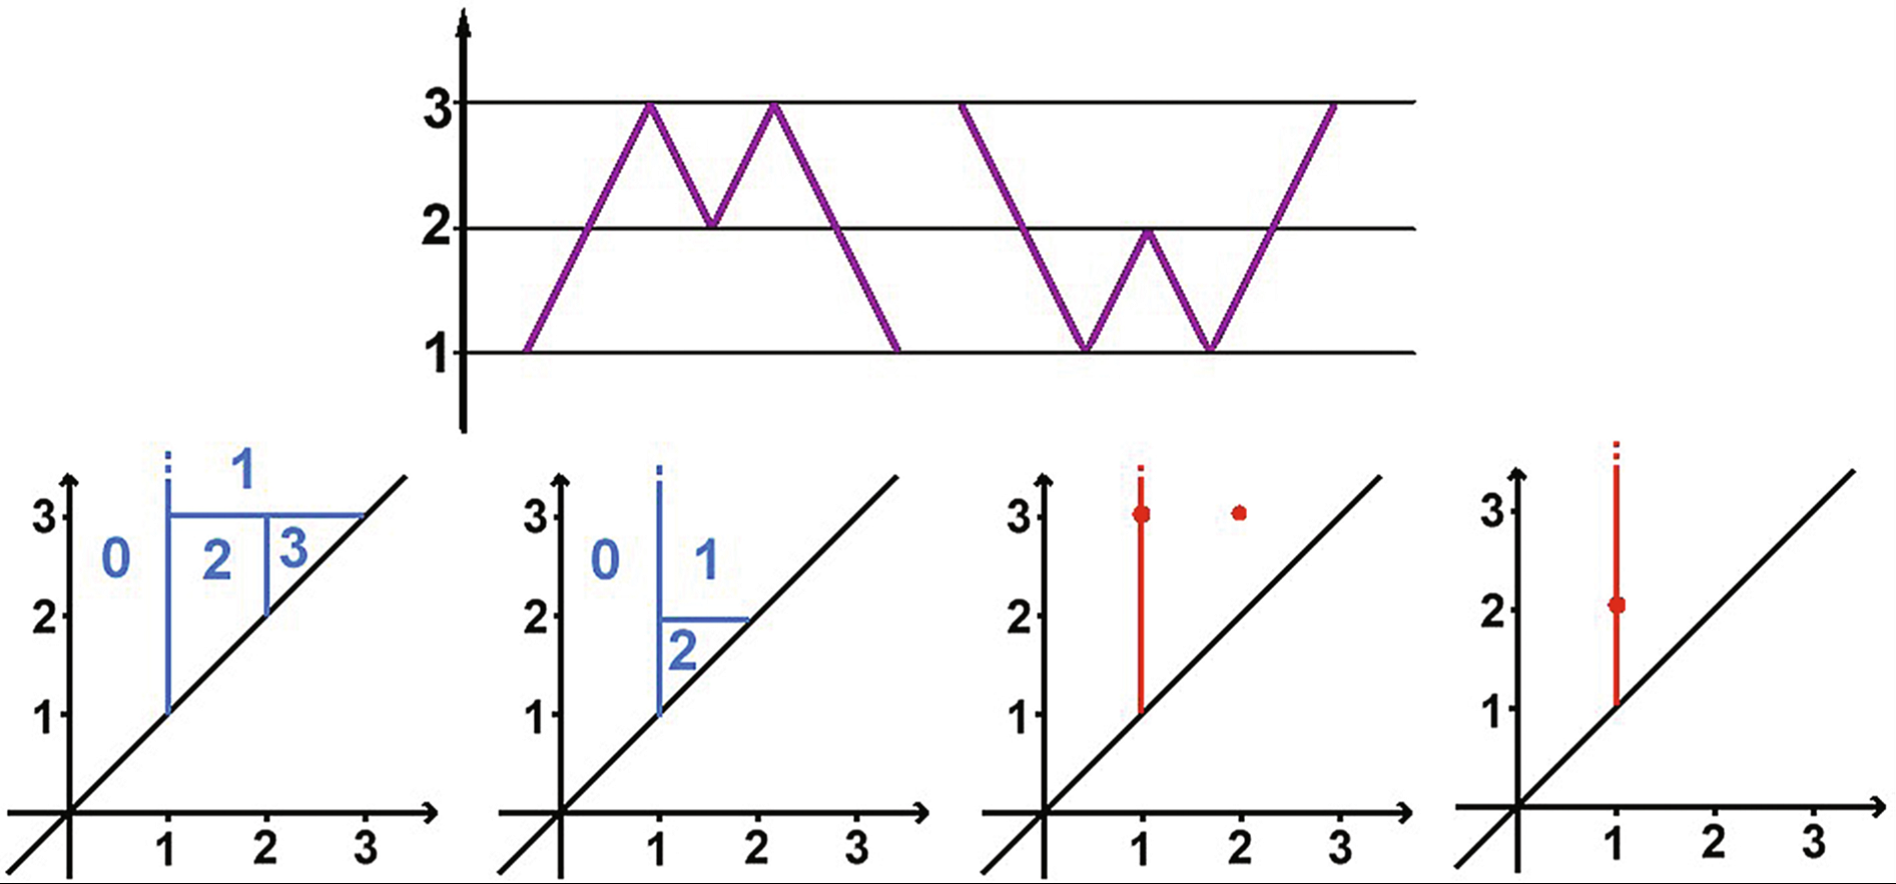
\includegraphics[height=5.5cm]{M_W 0-PBN 0-PDs.png}
\caption{$0$-PBN functions (on the left) e $0$-persistence diagrams (on the right) for $M$ and $W$.}\label{fig:M_W}
\end{figure}

\noindent We now want to determine the $0$-PBN functions and $0$-persistence diagrams for $M$ e $W$. So, we focus on the path-connected components of their sublevel sets as the height varies. 

\noindent For $M$, at height $l = 1$ two connected components arise and persist for heights $l<3$. A third one arises at height $l=2$ and merges with the others at height $l=3$, when only one component persists.

\noindent For $W$, at height $l = 1$ two connected components arise, persist for heights $1 \leq l <2$ and merge at height $l=2$, when only one component persists.

Thus, the different $0$-PBN functions and $0$-persistence diagrams we obtained, see figure~\ref{fig:M_W}, associated with the sublevel sets filtration of $M$ and $W$, allow one to distinguish the two objects, which are indistinguishable from a purely topological point of view.

\section{Persistence Images}
\label{PIs}

The introduction of persistence images in [Ada+17] is due to the need to solve the problem which is summarized in the following statements:

``How can we represent a persistence diagram so that: \\
(i) the output of the representation is a vector in $\mathbb{R}^n$, \\
(ii) the representation is stable with respect to input noise, \\
(iii) the representation is efficient to compute, \\
(iv) the representation maintains an interpretable connection to the original persistence diagram, and \\
(v) the representation allows one to adjust the relative importance of points in different
regions of the persistence diagram.''

It is possible to construct a finite-dimensional-vector representation of a persistence diagram called a {\bf persistence image} (PI). We first map a persistence diagram $B$ to an integrable function $\rho_B: \mathbb{R}^2 \rightarrow \mathbb{R}$ called a {\bf persistence surface}. The surface $\rho_B$ is defined as a weighted sum of probability density functions, typically Gaussian functions, one centered at each point in $B$.  The idea of persistence surfaces has already appeared even  before the development of persistent homology in [Fer+98] and [DFL98]. Taking a discretization of a subdomain of $\rho_B$ defines a grid. A persistence image, i.e., a matrix of pixel values, can be created by computing the integral of $\rho_B$ on each grid box. This PI is ``vectorization'' of the persistence diagram, and provides a solution to the problem statement above, as explained in detail in [Ada+17].

Precisely, let $B$ be a persistence diagram in birth-death coordinates.  Let $T : \mathbb{R}^2 \rightarrow \mathbb{R}^2$ be the linear transformation $T(u, v) = (u, v - u)$, and let $T(B)$ be the transformed set in birth-persistence coordinates, where each point $(u, v) \in B$ corresponds to a point $(u, v - u) \in T(B)$.

Let $\phi : \mathbb{R}^2 \rightarrow \mathbb{R}$ be a differentiable probability distribution with mean $m = (m_u, m_v) \in \mathbb{R}^2$. In applications, this distribution is usually chosen to be the normalized symmetric Gaussian $\phi_m = g_m$ with mean $m$ and variance $\sigma^2$, defined as
 
$$g_m(u, v) = \frac{1}{2\pi \sigma^2}e^{-\frac{[(u- m_u)^2+(v- m_v)^2]}{2\sigma^2}}.$$

We fix a non-negative weighting function $f: \mathbb{R}^2 \rightarrow \mathbb{R}$ that is zero along the horizontal axis, continuous, and piecewise differentiable. With these ingredients, we transform the persistence diagram into a scalar function over the plane.

\begin{defin} For $B$ a persistence diagram, the corresponding \textit{persistence surface} $\rho_B : \mathbb{R}^2 \rightarrow \mathbb{R}$ is the function 
$$ \rho_B(z) = \sum_{w \in T(B)} f(w)\phi_w(z)$$ \end{defin}

The reason for choosing differentiable distributions is we want to ``smooth out'' any ``jumps'' between values assumed on different points of B, blurring the transition between values around different cornerpoints.

The weighting function $f$ is critical to ensure the transformation from a persistence diagram to a persistence surface is stable: for the proof, we refer the reader to [Ada+17].
Finally, the surface $\rho_B(z)$ is reduced to a finite-dimensional vector by discretizing a relevant
subdomain and integrating $\rho_B(z)$ over each region in the discretization. In particular,
we fix a grid in the plane with n boxes (pixels) and assign to each the integral of $\rho_B$ over
that region.

\begin{defin}For $B$ a persistence diagram, its \textit{persistence image} is the collection of pixels $$I(\rho_B)_p = \iint_p \rho_B(u,v) \,dv\,du $$\end{defin}

When generating a PI, the user makes three choices: the resolution, the distribution
(and its associated parameters), and the weighting function. A strength of PIs is that they
are flexible; a weakness is that these choices are non-canonical. The interested reader in a more in-depth discussion of these aspects can refer to [Ada+17]



\chapter{A Persistence-Image-Based Approach for Music Information Retrieval}

The GTZAN dataset [TC02] is a widely used dataset for validating music genre recognition algorithms. We relied on MFCCs~\ref{MFCCs} as basic audio descriptors. Then, building on top of the MFCC-based representation, we leveraged Topological Data Analysis (TDA) and Persistent Homology (PH) to create more robust and concise descriptors.

In this chapter, we describe how we extracted and analyzed features from audio tracks of the GTZAN dataset. First we analyzed the extracted information performing a sublevel sets filtration on MFCCs and compute their $0$-persistence diagrams (PDs). The filtration is performed, as in subsection~\ref{example}, using \textit{height} as a filtering function, based on the number of independent $0$-cycles of MFCCs' sublevel sets, that is, the number of path-connected components. After computing the PDs, we considered the corresponding PIs, see section~\ref{PIs}, and applied appropriate machine learning techniques to learn how to appropriately associate a class (music genre) to a given PI.  

Let us first give an overview of the GTZAN, before describing in detail TDA computations and machine learning techniques we applied for our classification purposes.



\section{The GTZAN dataset}


\begin{table}[htbp]
\caption{Artist composition and Top Tags of each GTZAN category.}\label{fig:GTZAN_artists_tags}
\resizebox{\columnwidth}{!}{\begin{tabular}{|c|c|c|c|c|c|}
\hline
\bf Genre & blues & classical & country & disco & hiphop\\
\hline
\rule[-5cm]{0mm}{1cm}
\makecell{{\bf Artists} \\ (Percentage)} & \makecell{Robert Johnson (15-20),\\Hot Toddy (10-15),\\John Lee Hooker (10-15),\\Clifton Chenier (10-15),\\ Buckwheat Zydeco (10),\\Kelly Joe Phelps (10),\\Magic Slim and The Teardrops (10),\\Stevie Ray Vaughan (10)} & \makecell{Mozart (15-20),\\JS Bach (10-15),\\Vivaldi (10-15),\\FJ Haydn (5-10),\\ Percy Grainger (< 10),\\Franza Schubert (< 5),\\Claude Debussy (< 5),\\Maurice Ravel (<5),\\Henri Dutilleux (<5),\\Leonard Bernestein (<5),\\Beethoven (<5)} & 
\makecell{Willie Nelson (15-20),\\Vince Gill (10-15), Brad Paisley(10-15),\\ George Strait (< 5)} & 
\makecell{KC and The Sunshine Band (5-10),\\The Gibson Brothers (<5),\\Gloria Gaynor (<5),\\Ottawan (< 5)} & 
\makecell{A Tribe Called Quest (20),\\Bestie Boys (15-20),\\Public Enemy (15-20),\\Cypress Hill (< 5),\\Wu-Tang Clan(<5)}\\
\hline
\rule[-4mm]{0mm}{1cm}
\makecell{{\bf Top Tags} \\ (Percentage)} & 
\makecell{blues (25-30),\\zydeco (5-10),\\bluesrock (<5),\\swing (<5)\\swingblues (<5),\\cajun(<5)} &
\makecell{classical (30-35),\\ composer (5-10),\\composers (<5),\\instrumental (<5),\\baroque (<5)} &
\makecell{country (30),\\classic-country (5-10),\\oldies (<5),\\willienelson (<5)\\myfavourite (<5),\\vincegill (<5),\\vincegill (<5),\\greatsong (<5),\\ beautiful (<5),\\ outlawcountry (<5),\\ americana 60s (<5),\\ singer-songwriter (<5)\\} &
\makecell{disco (15-20),\\70s (5-10),\\pop (<5),\\80s (<5)\\dance (<5),\\funk (<5),\\soul (<5)} &
\makecell{hiphop (25),\\rap (10),\\ 90s (<5),\\oldschool (<5)\\80s (<5),\\gangstrap (<5),\\alternative (<5),\\beastieboys (<5),\\ a tribe call quest (<5),\\ political (<5),\\ RnB (<5),\\ New York (<5),\\ soul (<5)} &
\hline
\bf Genre & jazz & metal & pop & reggae & rock\\
\hline
\rule[-1cm]{0mm}{1cm}
\makecell{{\bf Artists} \\ (Percentage)} & \makecell{Coleman Hawkins (25-30),\\Joe Lovano (10-15),\\James Carter (5-10),\\Branford Marsalis Trio (5-10),\\ Miles Davis (<5),\\Joe Henderson (<5),\\Dexter Gordon (<5)} &
\makecell{Dio (10-15),\\New Bomb Turks (10-15),\\Metallica (<5),\\Iron Maiden (<5),\\ Dark Tranquillity (<5),\\Black Sabbath (<5),\\Rage Against The Machine (<5)} & 
\makecell{Britney Spears (20-25),\\Mandy Moore (5-10),\\Destiny's Child (5-10),\\Christina Aguilera (5-10),\\ Alanis Morissette (<5),\\Janet Jackson (<5),\\Jennifer Lopez (<5),\\ Mariah Carey (<5), \\ Celine Dion (<5)} & 
\makecell{Bob Marley (30-35),\\Dennis Brown (5-10),\\Prince Buster (5-10),\\Burning Spear (<5),\\ Gregory Isaacs (<5)} &
\makecell{Queen (10),\\Led Zeppelin (10-15),\\Morphine (10),\\The Stone Roses (5-10),\\ Simple Minds (5-10),\\Simply Red (5-10),\\The Rolling Stones (5-10),\\ Sting (5-10), \\ Jethro Tull (5-10),\\Survivor (5-10),\\Ani Di Franco (5-10)}\\
\hline
\rule[-4mm]{0mm}{1cm}
\makecell{{\bf Top Tags} \\ (Percentage)} & 
\makecell{jazz (25-30),\\saxophone (5-10),\\contemporaryjazz (<5),\\smooth-jazz (<5)\\jamescarter (<5),\\bebop (<5)} &
\makecell{heavy-metal (10-15),\\rock (5-10),\\hardrock (5-10),\\metal (5-10),\\classic-rock (<5),\\trashmetal(<5),\\punk (<5),\\80s(<5),\\punkrock (<5),\\melodic-death-metal (5-10)} &
\makecell{pop (15-20),\\female vocalist (5-10),\\dance (<5),\\RnB (5)\\90s (<5),\\Britney Spears (<5),\\rock (<5),\\soul (<5),\\ love (<5),\\ female vocalist (<5),\\ destiny's child (<5),\\soundtrack (<5),\\ female (<5)} &
\makecell{reggae (30-35),\\rootsreggae (5-10),\\ska (5),\\Bob Marley (<5),\\dancehall (<5)} &
\makecell{rock (10-15),\\classic rock (5-10),\\80s (<5),\\indie (<5)\\pop (<5),\\alternative (<5),\\hardrock (<5),\\british (<5), britpop (<5),\\ 70s (<5),\\ 90s (<5),\\progressive rock (<5),\\new wave (<5),\\indie-rock (<5)} &
\hline
\end{tabular}}\end{table}

\\

The gtzan8 audio dataset [TC02] contains 1000 tracks of 30-second length. Tracks are labelled according to ten genres, each containing 100 tracks which are all 22050Hz Mono 16-bit audio files in .wav format. The genres are blues, classical, country, disco, hip-hop, jazz, metal, pop, reggae, rock.

The dataset was introduced in 2002 and appears in at least 100 published works. It is the most-used public dataset in machine listening research for music genre recognition. Though its use is so widespread, GTZAN has always been missing metadata identifying its contents, until [Stu12] provided them for the first time.

In [Stu13] a partial reconstruction of GTZAN's excerpts is provided and is schematized in table~\ref{fig:GTZAN_artists_tags}. Furthermore, in the same article, the ways people describe the music or artist of each excerpt are surveyed, querying the application programming interface provided by last.fm, and retrieving the tags, also shown in table~\ref{fig:GTZAN_artists_tags}. 

The reader is referred to [Stu13] for a detailed discussion of limits and faults of GTZAN for MIR, particularly for music genre recognition.

\paragraph{Data folders}
\begin{itemize}
    \item ``genres original''. A collection of ten genre folders with 100 audio files each, all having a length of 30 seconds.
    \item ``images original''. For each audio file, a visual representation of the corresponding Mel spectrogram.
    \item Two CSV files containing features of the audio files. One file has for each song mean and variance computed over multiple features that can be extracted from an audio file. The other file has the same structure, but each song is split into three-seconds audio files.
\end{itemize}

\section{The steps to PIs computation}

We now describe in detail the steps we performed to extract features from the GTZAN’s tracks, analyze them with TDA tools, and classify the TDA-based signatures with machine learning methods. We provide the Python code of the algorithms we devised in Appendix~\ref{appendix}.

\paragraph{Feature extraction}

\begin{figure}[tb]
\centering
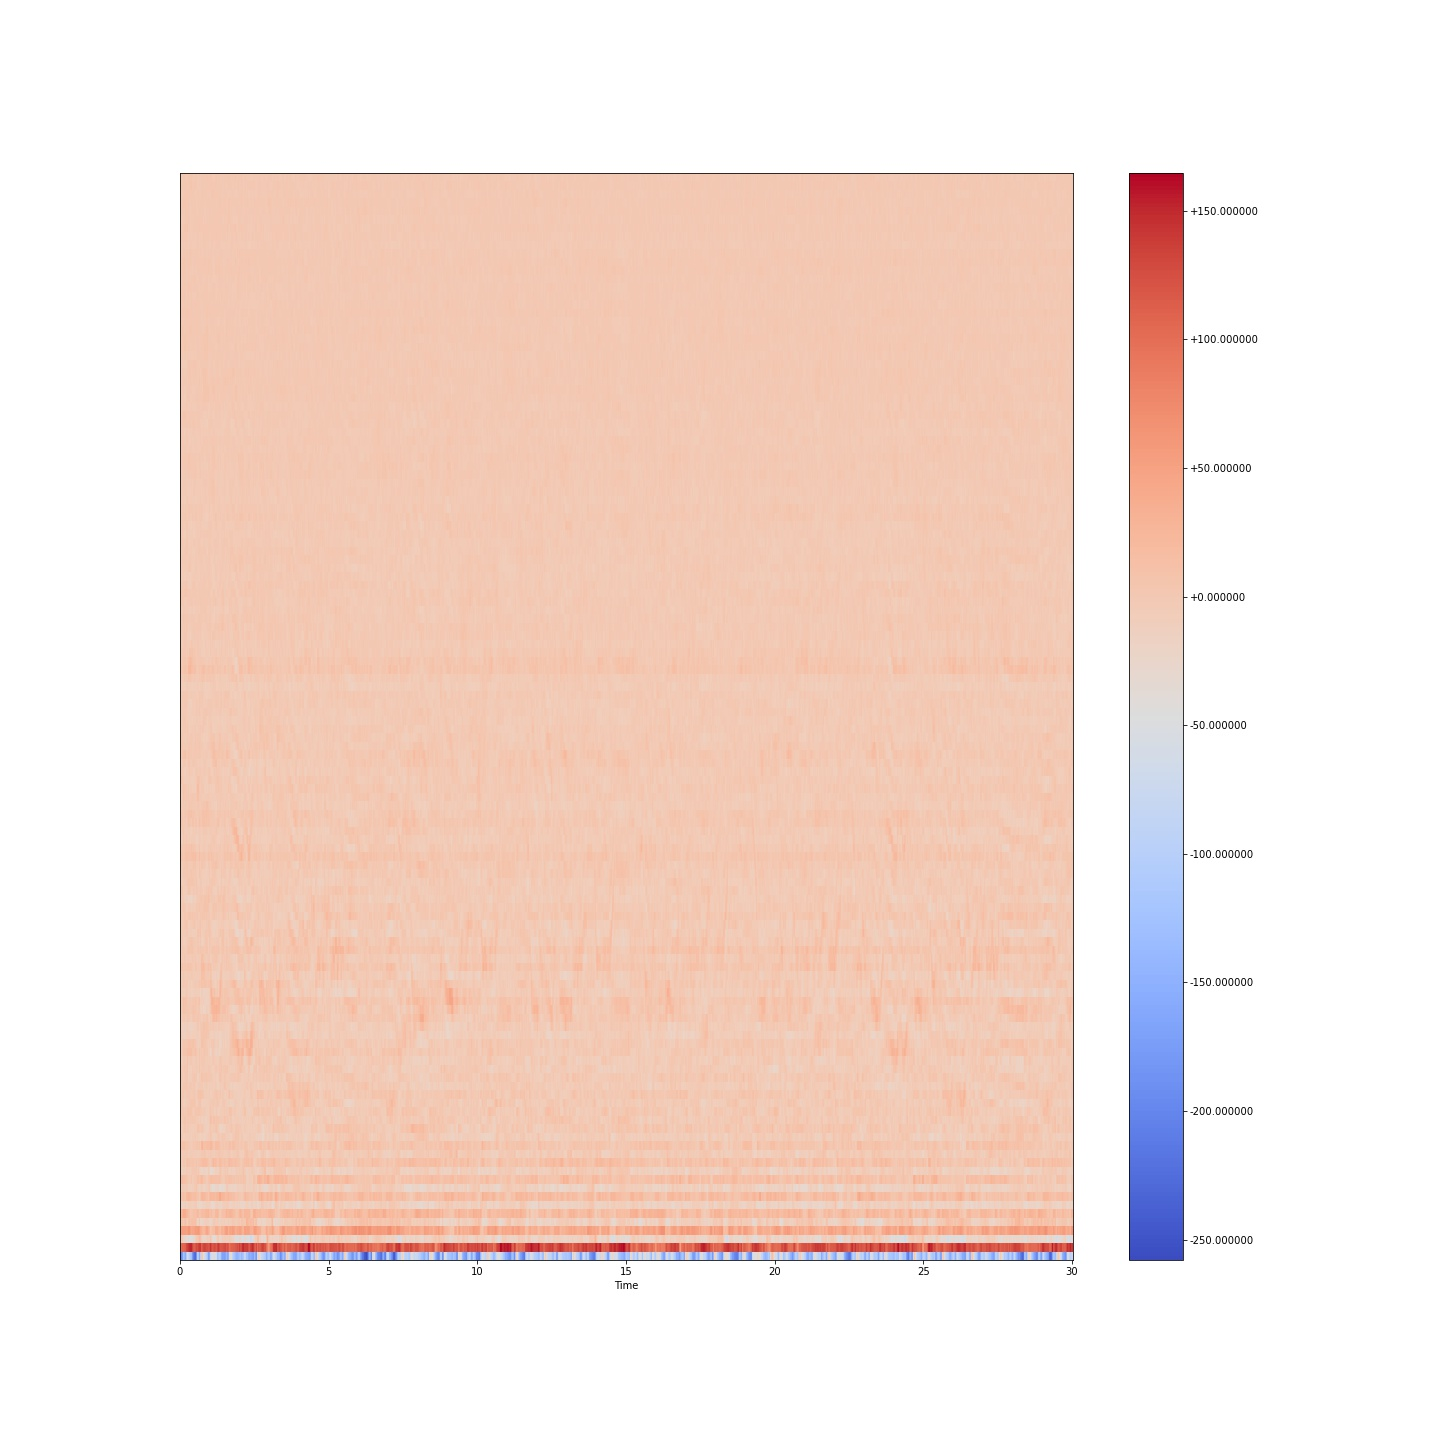
\includegraphics[height=10cm]{testplot.jpg}
\caption{An example of visualization of MFCCs extracted from audio file blues.00000 from the blues folder of GTZAN recognized as \textit{One Bourbon, One Scotch, One Beer} by John Lee Hooker.}\label{fig:MFCCs_plot}
\end{figure}

The first step concerns the extraction of MFCCs from audio tracks. We used the Python library \textit{Librosa} [McF+21]’s function librosa.feature.mfcc, which generates MFCCs from a audio signal. For each track we set the sample rate parameter \textit{sr} to the value we read by loading the sampling rate with librosa itself, and we set to 128 the parameter \textit{n\_mfcc}, the number of MFCCs to be computed. 

The Librosa’s function \textit{librosa.display.specshow} allows one to visualize the input data. In figure~\ref{fig:MFCCs_plot} we report a visualization of MFCCs of a track from the ``blues’’ folder. 

\paragraph{Sublevel sets filtrations and $0$-PDs}
Once we obtained MFCCs of all the audio tracks, we performed their sublevel sets filtrations, using the special function \textit{lower\_star\_img} imported from the Python package \textit{Ripser} [TSB18]. It returns the $0$-PDs associated with the filtrations, stored as NumPy arrays with shapes $(-,2)$.
The machine interprets as infinity the ordinates of cornerlines or cornerpoints with very big death-coordinates. Therefore, in each PD it is necessary to replace these elements with cornerpoints having the same abscissa and ordinate equal to the maximum finite non-NaN life plus one of all the cornerpoints in the diagram. So, given a cornerline - or a cornerpoint having a too much big or NaN death-coordinate - with abscissa $w$, we replaced it with the point $$(w, max \{v : (u, v) \ is \ a \ proper \ cornerpoint,\ v \ is\ not\ a\ NaN\}+1).$$

\begin{figure}[tb]
\advance\leftskip-8cm
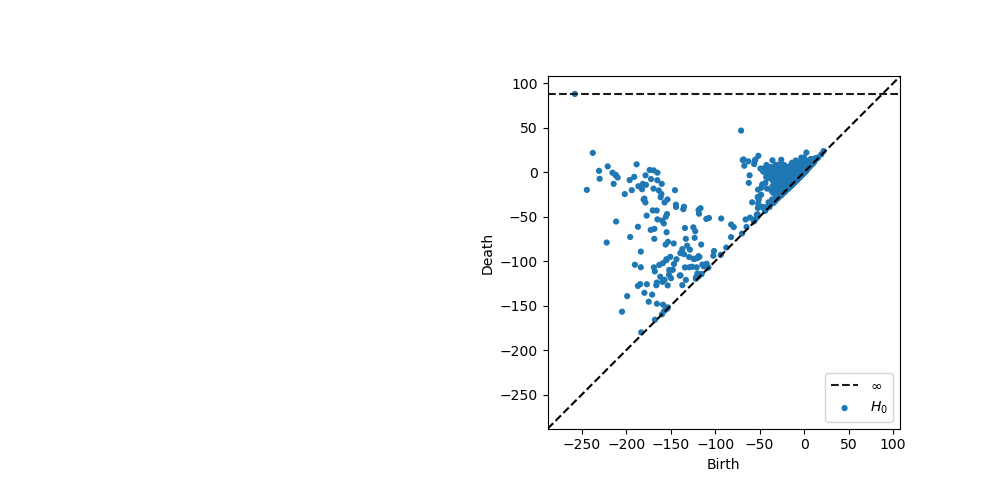
\includegraphics[height=10cm]{0-PD.png}
\caption{The $0$-PD corresponding to the sublevel sets filtration of MFCCs in figure~\ref{fig:MFCCs_plot}.}\label{fig:0-PD}
\end{figure}

\paragraph{PIs computation} We then wanted to obtain the PIs corresponding to the $0$-PDs, according to section~\ref{PIs}. We computed them with the function \textit{PersistenceImager} imported from the Python package \textit{Persim}. It provides a \textit{fit} method, which can be called on one or more NumPy arrays to automatically determine the minimum birth and persistence ranges needed to capture all persistence pairs. The ranges and resolution are automatically adjusted to accommodate the specified pixel size. Once we have $0$-PDs associated with MFCCs’ filtrations we can fit them and then generate PIs with the \textit{trasform} method, which can be called on the fitted diagrams to generate the corresponding PIs, also stored as NumPy arrays.

\begin{figure}[tb]
\centering
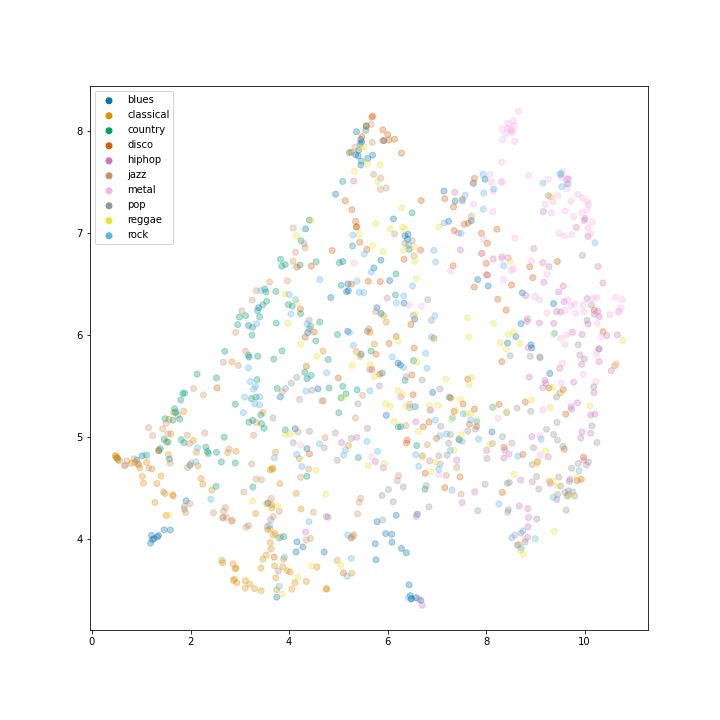
\includegraphics[height=10cm]{umap_genres.png}
\caption{UMAP scatter plot of PIs' projection.}\label{fig:UMAPlot}
\end{figure}

 
\paragraph {PIs visualization} Having fitted the $0$-PDs before computing the corresponding PIs, their shapes are likely all the same or very similar to each other. However, we reshaped them to the shape of a PI with the minimum number of elements in each dimension of all computed PIs and we obtained PIs with shapes $(763,768)$. We can thus think of PIs as points of a submanifold of $\mathbb{R}^{763\times768}$. The UMAP algorithm for dimension reduction [MHM20] allowed us to visualize their projections on a plane, see figure~\ref{fig:UMAPlot}, to try to guess any regularity in their distribution with respect to how they are divided per genre. Before performing the projection, we need to flatten the arrays representing PIs with the \textit{.flatten} method, that is, creating a copy of each array collapsed into one row. Then we can fit the flattened arrays with the UMAP \textit{fit} method and transform them with the UMAP \textit{transform} method for dimension reduction.\\

\section{Classification and cross-validation}


We need to check the validity of our approach for MIR, in particular for music genre recognition, by trying an automatic classification with a machine learning pipeline, comparing the accuracy we obtain by applying it first to the starting dataset and then to the PIs.

For our automatic classification problem we used Support-vector Machines (SVMs). SVMs are supervised learning methods used for classification and regression [Ped+11]. These robust prediction methods based on statistical learning frameworks were introduced in [BGV92] in the 1990s\footnote{A good reference for a brief introduction is also [EP99].}.

The machine learning library \textit{Scikit-learn} [Ped+11] provides classes capable of performing binary and multi-class classification on a dataset. We used \textit{SVC} (Support Vector Classification)\footnote{For the mathemtical formulation the reader can also refer to [Ped+11].}.

To avoid overfitting, it is common practice, when performing a machine learning experiment, to hold out part of the available data as a test set $X_{test}, y_{test}$. The problem remains that the results may depend on a particular random choice for the pair of sets (train, validation). A solution to this problem is a procedure called cross-validation (CV). In the basic approach, called $k$-fold CV, the training set is split into $k$ smaller sets and the following procedure is followed for each of the $k$ “folds”\footnote{See [Ped+11] for a more in-depth discussion.}:
\begin{itemize}
    \item A model is trained using $k-1$ of the folds as training dataset;
    \item the resulting model is validated on the remaining part of the dataset (i.e., it is used as a testing dataset to compute a performance measure such as accuracy).
\end{itemize}

\noindent In particular, we used \textit{Stratified k-fold} for cross-validation of SVC on our datasets. 

\noindent We set the number of folds to 5.

A figure follows representing the flow of the algorithm:
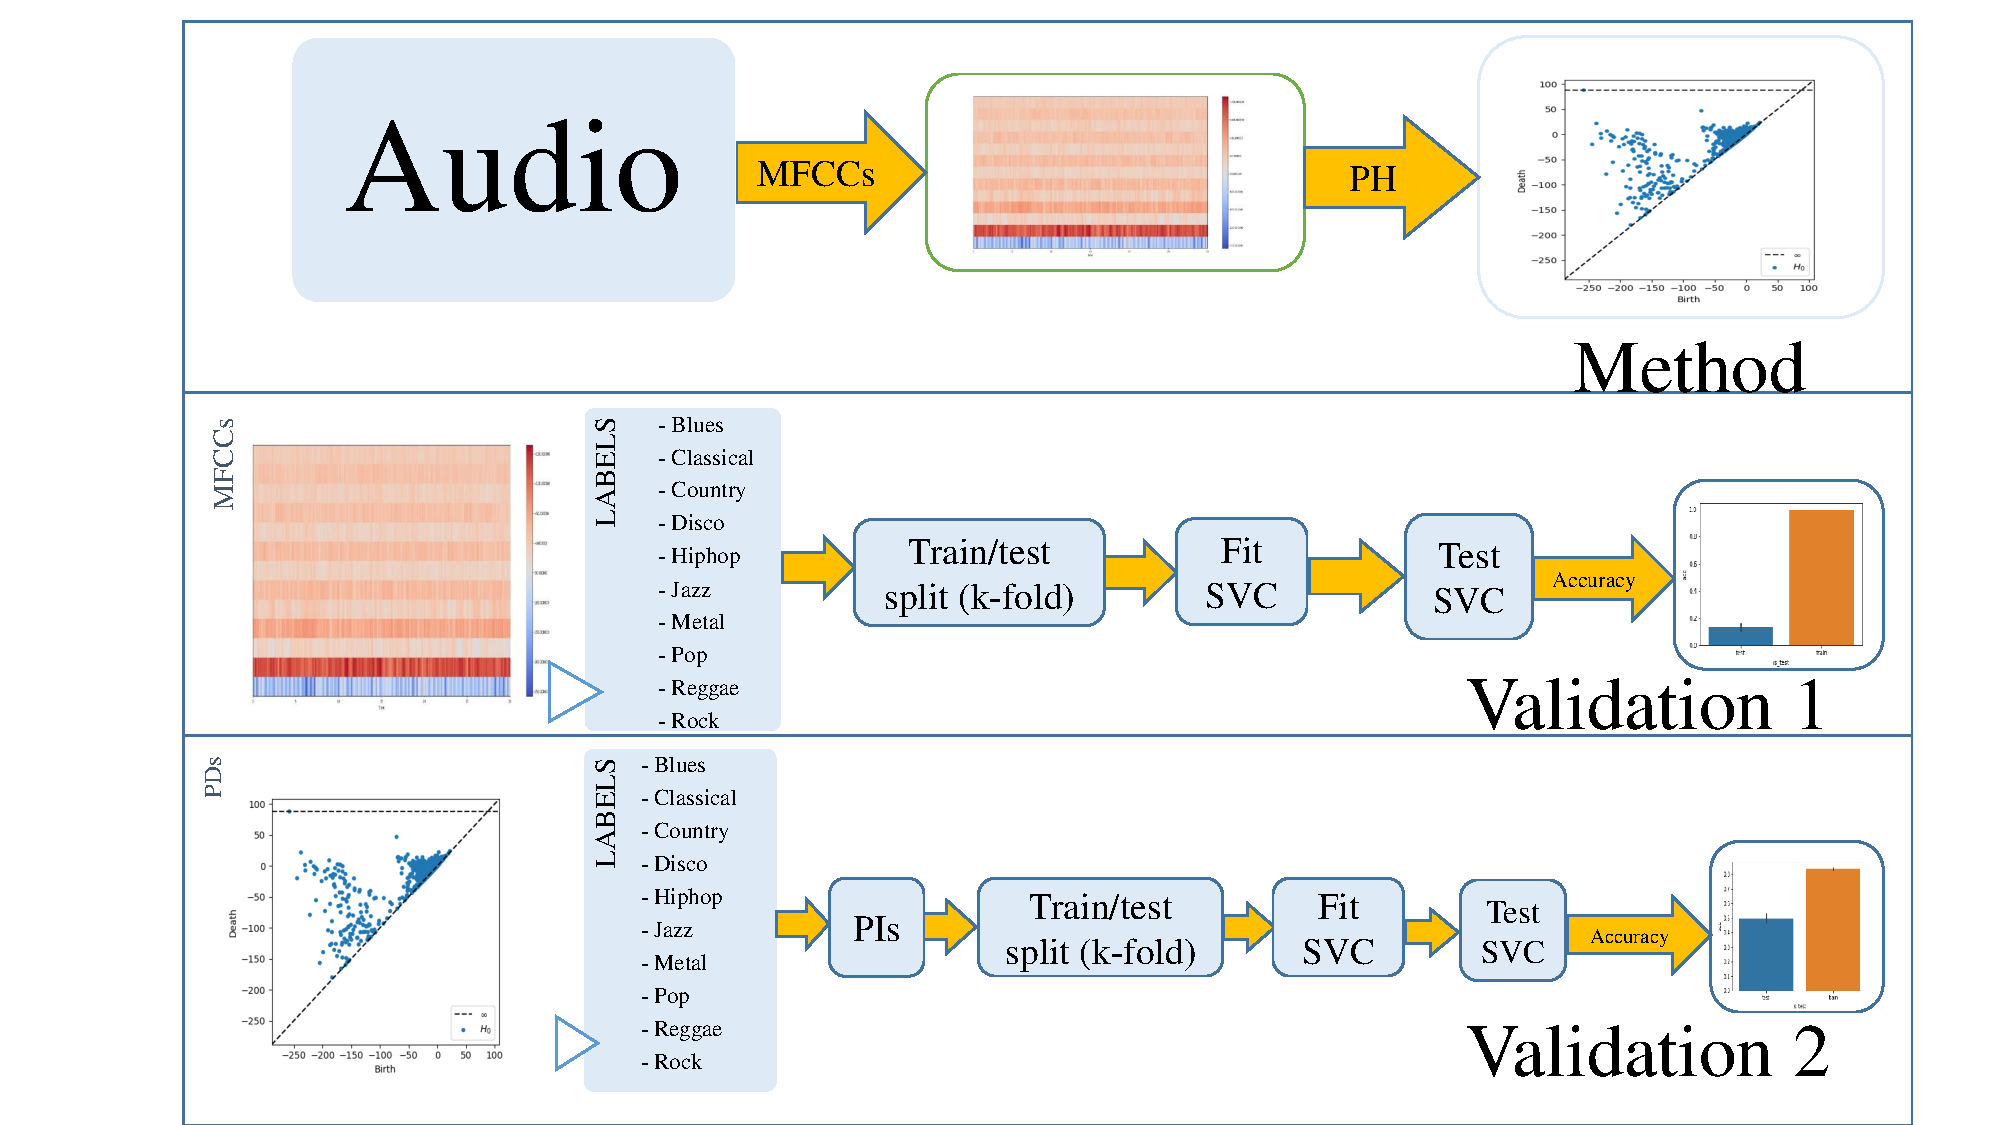
\includepdf[pages=-]{FLOWCHART thesis.pdf}



\section{Results}

We report \textit{confusion matrices} and {accuracies} we obtained applicating the model SVC both to MFCCs and then to PIs, with music genres as classes. In a confusion matrix, the columns correspond to the actual class and the rows to the predicted class. By definition, the element on row $i$ and column $j$ is the number of cases in which the classifier classified the ``true'' class $i$ as class $j$.
 
The accuracy is obtained as the number of classes that the classifier correctly predicts divided by the total number of predictions made.
The \textit{train accuracy} is the accuracy of a model on examples it was constructed on. The \textit{test accuracy} is the accuracy of a model on examples it hasn't seen.

A confusion matrix obtained for a testing set of MFCCs:\\
\begin{pmatrix}
0 & 20 & 0 & 0 & 0 & 0 & 0 & 0 & 0 & 0\\
0 & 20 & 0 & 0 & 0 & 0 & 0 & 0 & 0 & 0\\
0 & 20 & 0 & 0 & 0 & 0 & 0 & 0 & 0 & 0\\
0 & 20 & 0 & 0 & 0 & 0 & 0 & 0 & 0 & 0\\
0 & 20 & 0 & 0 & 0 & 0 & 0 & 0 & 0 & 0\\
0 & 20 & 0 & 0 & 0 & 0 & 0 & 0 & 0 & 0\\
1 & 11 & 6 & 0 & 0 & 0 & 0 & 0 & 0 & 2\\
0 & 20 & 0 & 0 & 0 & 0 & 0 & 0 & 0 & 0\\
0 & 20 & 0 & 0 & 0 & 0 & 0 & 0 & 0 & 0\\
0 & 16 & 3 & 0 & 0 & 0 & 1 & 0 & 0 & 0

\end{pmatrix}$
\\
A confusion matrix obtained for a training set of MFCCs:\\
$\begin{pmatrix}
80 & 0 & 0 & 0 & 0 & 0 & 0 & 0 & 0 & 0\\
0 & 80 & 0 & 0 & 0 & 0 & 0 & 0 & 0 & 0\\
0 & 0 & 80 & 0 & 0 & 0 & 0 & 0 & 0 & 0\\
0 & 0 & 0 & 80 & 0 & 0 & 0 & 0 & 0 & 0\\
0 & 0 & 0 & 0 & 80 & 0 & 0 & 0 & 0 & 0\\
0 & 0 & 0 & 0 & 0 & 79 & 0 & 0 & 0 & 0\\
0 & 0 & 0 & 0 & 0 & 0 & 80 & 0 & 0 & 0\\
0 & 0 & 0 & 0 & 0 & 0 & 0 & 80 & 0 & 0\\
0 & 0 & 0 & 0 & 0 & 0 & 0 & 0 & 80 & 0\\
0 & 0 & 0 & 0 & 0 & 0 & 1 & 0 & 0 & 80
\end{pmatrix}$
\\

A confusion matrix obtained for a testing set of PIs:\\

$\begin{pmatrix}
3 & 0 & 2 & 2 & 0 & 4 & 0 & 7 & 2 & 0\\
0 & 17 & 3 & 0 & 0 & 0 & 0 & 0 & 0 & 0\\
1 & 0 & 9 & 0 & 0 & 3 & 0 & 2 & 0 & 5\\
0 & 0 & 2 & 9 & 0 & 0 & 0 & 4 & 1 & 4\\
0 & 0 & 0 & 1 & 15 & 0 & 2 & 0 & 2 & 0\\
2 & 3 & 7 & 0 & 0 & 7 & 0 & 0 & 0 & 1\\
0 & 0 & 0 & 1 & 3 & 0 & 13 & 0 & 2 & 1\\
0 & 2 & 2 & 1 & 0 & 1 & 0 & 10 & 0 & 4\\
4 & 0 & 1 & 3 & 1 & 0 & 0 & 0 & 10 & 1\\
1 & 0& 4 & 0 & 0 & 1 & 4 & 1 & 4 & 5
\end{pmatrix}$
\\


A confusion matrix obtained for a training set of MFCCs:\\
$\begin{pmatrix}

61 & 2 & 3& 5 & 1& 3 & 0 & 1 & 0 & 4\\
0 & 76 & 2 & 0 & 0 & 0 & 0 & 0 & 0 & 2\\
0 & 0 & 75 & 0 & 0 & 0 & 0 & 0 & 0 &5\\
1 & 1 & 2 & 67 & 1 & 0 & 0 & 2 & 1 & 5\\
0 & 0 & 0 & 0 & 74 & 3 & 0 & 2 & 0 & 1\\
2 & 5 & 5 & 1 & 0 & 60 & 0 & 1 & 0 & 5\\
0 & 0 & 0  & 0 & 0 & 0 & 75 & 0 & 0 & 5\\
0 & 0 & 4 & 0 & 3 & 0 & 1 & 70 & 0 & 2\\
0 & 2 & 1 & 0 & 2 & 0 & 0 & 3 & 72 & 0\\
3 & 2& 13 & 4 & 0 & 3 & 3 & 2 & 0 & 50

\end{pmatrix}$
\\

\begin{figure}[tb]
\centering
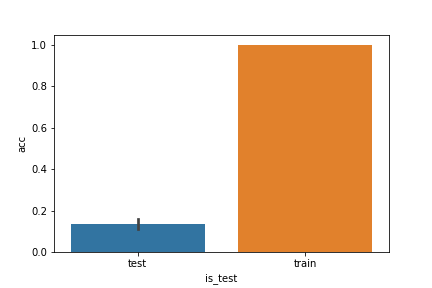
\includegraphics[height=5cm]{mfccs_accuracy_barplot.png}
\caption{An estimate of the central tendency for test and train accuracy of SVC through the 5 fits in which it is implemented on MFCCs.}\label{fig:acc_plot_MFCCs}
\end{figure}

\begin{figure}[tb]
\centering
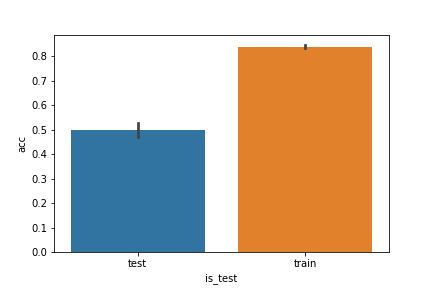
\includegraphics[height=5cm]{PIs_accuracy_barplot.png}
\caption{An estimate of the central tendency for test and train accuracy of SVC through the 5 fits in which it is implemented on PIs.}\label{fig:acc_plot_PIs}
\end{figure}

In figures~\ref{fig:acc_plot_MFCCs} and~\ref{fig:acc_plot_PIs}, bar plots representing train and test accuracies for SVC performed on MFCCs and on PIs respectively. 

The significant improvement obtained in the test accuracy by performing a standard classifying method as SVC on PIs with respect to MFCCs is in favor of the validity of our theory: the functor that maps the image (MFCCs), thought as a topological space, in the persistence modules is necessary to extract information, which would otherwise be drowned in noise.

\chapter{An alternative approach for feature extraction: cardinality reduction with the ``Ziggurat'' algorithm for cornerpoints selection}

We are currently working on an alternative tool that we would like to apply for our MIR classification purposes. However, this research work is still ongoing. Therefore, in this chapter, we aim to expose and analyze some preliminary results relating to the application of the algorithm we are working on.
Instead of considering the persistence images corresponding to PDs, we consider for each diagram $D$ a subdiagram $D'$ of relevant cornerpoints selected through an algorithm called Ziggurat, introduced in [Gur21]; the working hypothesis is to think of $D'$ as the ``reconstruction'' of what we acquired in $D$, restoring any symmetry lost during the extraction of the information, and thus removing ``noise'' from $D$. In the next sections, largely built on the work done in [Gur21], we are going deeper into the details of the algorithm.

\section{Cornerpoints selection}
\label{Cornerpoint selection}

Given a pair $(X, f)$, $k$-persistent Betti numbers functions ($k$-PBN) and $k$-persistence diagrams
($k$-PD) have been defined in Chapter 1. These mathematical tools turn out very useful because they represent a sort of digital imprint of the initial object, obtained by selecting particular interesting features  through
the filtering function $f$.
As we have seen, the persistence diagrams are formed by cornerlines and cornerpoints,
whose coordinates represent birth and death of $k$-cycles.
However, not all cornerpoints have the same relevance: if the starting object is complex - of  medical nature for instance 
 - part of cornerpoints could represent to noise.
Experimental evidence suggests that, in most cases, such cornerpoints are very close to the diagonal. It is possible that  
other cornerpoints associated with the result of
a disturbance in the initial object are also present.
Therefore, It is essential to make a selection of the most important cornerpoints, assigning to each one a certain degree of relevance, in order to obtain a hierarchical classification of all points.

Consider the figure~\ref{fig:filtration example}.
This context is similar to the example~\ref{example}. The starting object is represented on the left, while the corresponding $0$-persistence diagram is represented on the right, obtained through the filtering function "height". The \textit{elderly rule} is used to construct the diagram, that is, a $0$-cycle (path-connected component) is “killed" only
when it merges with another older $0$-cycle born earlier. For instance, the first $0$-cycle that is born is the one relating to the minimum point of the starting object, and it will never die because it is the oldest one. Such information is contained in the cornerline of abscissa $0$. Subsequently, the second $0$-cycle is born at height $1$ and it dies at altitude $23$. The other $0$-cycles are born
respectively at heights $5$, $10$ and $11$ and die at the heights indicated by ordinates of the corresponding cornerpoints.
In particular, the $0$-cycle represented by the cornerpoint $c$ arises at height $10$ and, immediately after, the one represented by cornerpoint $d$ is born at height $11$.
In this area of the starting object, we can notice a sudden alternation of maximum and minimum peaks, which indicate the presence of a disturbance with high probability. Analyzing the image better, the second oscillation can be considered as if it was negligible compared to the first, since this one "covers" the second, in a certain sense.
To take this into account, at the level of the persistence diagram,
we need to give less importance to the cornerpoint $d$, which represents the second oscillation, concerning $c$, which instead represents the first.
Furthermore, even if in this example there is no further noise, as previously anticipated, generally it would be necessary to assign less importance also to all cornerpoints close to the diagonal.

\section{Ziggurat}

\begin{defin} Let $D$ be a persistence diagram with a finite set of cornerpoints. Let us assume that all points on the diagonal belong to $D$. To make
the definition simpler, add a cornerpoint at $(-\infty, +\infty)$. 
Let us define the function \textit{legacy} $\eta: \mathbb{R}^2 \rightarrow \mathbb{R}$ such that $$\eta((u, v)) = max\{\overline{u} - \overline{v} \ | (\overline{u}, \overline{v}) \in D, \overline{u} \leq u, \overline{v} \leq v\}$$\end{defin}

\begin{defin} For $D$ a persistence diagram as above and $\eta$ legacy, \textit{Ziggurat} is defined as $$Z_D = \{(u, v, w) \in \mathbb{R}^3 | \eta((u; v)) > -\infty, w \leq \eta((u,v))\}$$.   \end{defin}

\noindent Once the Ziggurat has been obtained starting from the persistence diagram $D$, it is possible to perform its filtration using the $0$-persistence diagram $\mathcal{D}$ of the Ziggurat $Z_D$, obtained through the filtering function $f_{Z_D}(u, v, w) = u - v - w$.
To correctly interpret that, it is very convenient to
have a graphical display of the Ziggurat.

Before proceeding with its graphical construction, it is useful to give a more qualitative explanation of the Ziggurat structure. It develops in the three-dimensional space $\mathbb{R}^3$ and it is constructed starting from a persistence diagram $D$, which is instead represented in the two-dimensional space $\mathbb{R}^2$.
For example, we can refer to the $D$ persistence diagram in figure~\ref{fig:Ziggurat 2D}


Each cornerpoint with coordinates $(u, v)$ has persistence $v - u$, and, as defined in the persistence diagram, all persistences will always be positive.
To represent the Ziggurat graphically, many prisms are built with a
triangular base as many as there are cornerpoints. The upper base of each prism
is defined by the triangle generated starting from the vertical and
horizontal extensions on the bisector of the first quadrant of each cornerpoint. The upper base of the prisms is positioned at a height equal to the persistence of the
corresponding cornerpoint, with changed sign. Theoretically, every prism would have depth extending to $- \infty$, but, for graphical purposes, it is considered
a maximum depth equal to the highest persistence of the cornerpoints $+ 1$ (changing the sign), and the cornerlines $ (x, - \infty)$ are
replaced by cornerpoints with abscissa $x$ and ordinate equal to the maximum ordinate of other cornerpoints $+ 1$. Referring to figure~\ref{fig:Ziggurat 2D}, the
cornerpoint with the highest persistence is the one corresponding to the cornerline of abscissa $2$, whose coordinates are $(2, 15)$. This cornerpoint has a persistence 
$15-2 = 13$, and therefore the maximum depth of all prisms is $(13 + 1) =  14$.
An additional triangular prism is also added at $0$, with the upper base
constructed starting from the bisector of the first quadrant. In 
figures ~\ref{fig:Ziggurat 1}, ~\ref{fig:Ziggurat 2}, ~\ref{fig:Ziggurat 3} a first construction of the corresponding Ziggurat is represented
in the persistence diagram in figure~\ref{fig:Ziggurat 2D}, performed by Davide Gurrieri in [Gur21] using the software
CAD Creo Parametric.

Finally, the figure~\ref{fig:Ziggurat 3D} shows the front view of the Ziggurat cut from the plane corresponding to the level $k = 4$ of the filtering function $u - v - w$.



\subsection{Cornerpoints selection in the Ziggurat's persistence diagram}

\label{Ziggurat selection}


As previously mentioned, the idea behind the cornerpoints selection process in a persistence diagram $D$ is to use the pair $(Z_ {D}, f_ {Z_D})$, where $f_{Z_D}(u, v, w) = u - v - w$, an oblique plane which, at level $k = 0$, intersects all the prisms vertices of the Ziggurat $Z_D$. Therefore, the $0$-persistence diagram $\mathcal{D}$ generated by the pair $(Z_D, f_{Z_D})$ is used to obtain a relevance ranking of $D$'s cornerpoints. As $k>0$, the plane defined by $u-v-w = k$ moves parallel to itself, intersecting the prisms of the Ziggurat. Initially, the intersection generates $n$ pyramids, each corresponding to one of the $n$ cornerpoints of $D$. As $k$ increases, pyramids start to merge with each other, going to ``die''. Unlike the example in the figure~\ref{fig:filtration example}, in this filtration pyramids are all born at the same time. In fact, for $k = 0$, we have $u - v - w = 0$, hence $w = u - v$, which is the persistence of the cornerpoint $(u, v)$ changed in sign. Therefore, the plane intersects the prism associated with the cornerpoint $(u, v)$ at the point with coordinates $(u, v, u-v)$, corresponding by construction to the vertex of the upper base of the prism lying on the ``vertical'' line of $(u, v)$ itself, which is the vertex of the pyramid corresponding to $(u, v)$. Therefore, it is not possible to use the elderly rule as previously introduced. It was therefore decided to consider the pyramids with an old age order based on the persistence of the corresponding cornerpoints: the first pyramid to be born is the one with the highest persistence. Once assigned the order of birth, we proceed according to the \textit{elderly rule}: a pyramid dies when it merges with another pyramid born previously. In the case there are pyramids whose corresponding cornerpoints have the same persistence, the pyramid corresponding to the cornerpoint with the highest abscissa is considered to be older than the other one.

\noindent Also, by convention, a pyramid dies when it merges with
the plateau at height $0$. This allows attributing less relevance to cornerpoints close to the diagonal, which typically represent noise. To understand better the concepts exposed above, consider the persistence diagram of figure~\ref{fig:filtration example} where, for simplicity, the cornerline is neglected. Figures ~\ref{fig:Ziggurat 3D k=0}, ~\ref{fig:Ziggurat 3D k=2}, ~\ref{fig:Ziggurat 3D k=7}, ~\ref{fig:Ziggurat 3D k=10} show the birth and the death of pyramids for different values of $k$.

\noindent For $k>0$ all the
pyramids are born. As mentioned above, even if the pyramids are born at the same time,
one is considered older than another based on the persistence of the corresponding cornerpoints. Thus, the oldest pyramid is consider to be
$a$, followed by $c$, $d$, and $b$. Then we apply the elderly rule convention.
For $k = 2$ the pyramid $d$ dies merging with $c$. For $k = 7$ the pyramid $b$ dies merging with $d$ (and with the plateau at the same time). In the end, for $ k = 10$ the pyramid $c$ dies, merging with the plateau.
The oldest pyramid $a$ is considered to be never-dying, even if it would melt with the plateau for $ k = 22$. As a result of this operation, we obtain the $D$ persistence diagram in figure~\ref{fig:Ziggurat persistence diagram}, which provides the desired relevance ranking.

\noindent Referring to section~\ref{Cornerpoint selection}, we obtained that point $d$ had to be
considered less relevant, as it derives from a disturbance of the starting object. Therefore, the result obtained is coherent with our expectations: point $d$ is at the bottom of the relevance ranking and can be discarded.

\section{Selection Algorithm}

Now, it is necessary to automatize the selection operation via
an algorithm taking in input the coordinates and other attributes of the cornerpoints, and, for
each persistence diagram, returns the relevance ranking calculated as explained through the example of paragraph~\ref{Ziggurat selection}. The algorithm was designed in Python language. The code is
reported in the appendix~\ref{appendix B}.
Now, a theoretical explanation follows of how the algorithm works.
Let $D$ be a persistence plot consisting of $n$ cornerpoints with coordinates $(x_i, y_i)$, with $i = 1, \dots, n$. Consider the Ziggurat $Z_D$, starting at $D$ and
the plane $z = x - y - k$ as $k$ varies. A summary follows of the assumptions made to make the selection:
\begin{itemize}
    \item When a pyramid generated by a cornerpoint merges with the plateau, it is considered dead.
    \item To apply the elderly rule, it is assumed that a  cornerpoint is born before than another one if it has higher persistence.
    \item In the case two cornerpoints have the same persistence, it is considered to be older the cornerpoint with higher abscissa.
    \item By convention, the cornerpoint with the greatest persistence never dies (in the persistence diagram of $Z_D$ it becomes a cornerline).
\end{itemize}

\noindent Python language allowed us to treat cornerpoints as objects of a class characterized by different attributes: an identificative number (id), coordinates $(x, y)$, the level of the Ziggurat filtering function when the corresponding pyramid merges with another one for the first time, and multiplicity are the main ones. 

\noindent For simplicity, from now on we will say that a cornerpoint merges with another one, is younger/older than another one, persists or dies, meaning that the corresponding pyramid merges with another one, is younger/older than another one, persists or dies respectively.

\noindent As seen in paragraph~\ref{Ziggurat selection}, it is necessary to compute all $k_i$, with $i = 1, \dots n$, at which
the pyramids generated by the $n$ cornerpoints with coordinates $(x_i, y_i)$ die. 
A pyramid can die only if it merges with an older pyramid
or it merges with the plateau. Given a generic cornerpoint with coordinates $(xi, yi)$, to find the corresponding level $k_i$ (the attribute level defined in the function ``merging level'' in the code) it suffices to verify if this cornerpoint merges with  cornerpoints belonging to the following set: 
$$A_i = \{(x, y) \in \mathbb{R}^2 | y > x + (y_i - x_i), 
x> x_i - (y_i - xi),
y < y_i + (y_i - x_i), 
y < x + 2(yi - xi),

\
y = x + (y_i - x_i),   
x_i < x \leq y_i) \}$$

\

\noindent If a cornerpoint does not belong to $A_i$, it means
that it is younger than $(x_i, y_i)$, or it is older and has no time to merge with $(xi, yi)$ because $(x_i, y_i)$ has already merged with the plateau.
\noindent Comparing $(xi, yi)$ with any other cornerpoint $(x_h, y_h) \neq (x_i, y_i)$ we have:

\begin{itemize}
    \item If $(x_h, y_h) \not\in Ai$, then $k_{i,h} = yi - xi$
    \item If $(x_h, y_h) \in Ai$, then $$k_{i,h} = \left \{
    \begin{array}{lr}
    x_i - x_h & if \ (x_h, y_h) \in B_i\\
    y_h - y_i & if \ (x_h, y_h) \in C_i \\
    x_i - x_h + y_h - x_i & if \ (x_h, y_h) \in D_i \\
\end{array}\right.$$ 
\end{itemize}

where

\begin{itemize}
    \item $B_i = \{(x, y) \in \mathbb{R}^2 | y > x + (y_i - x_i), x > xi - (yi - xi), y \leq y_i\}$
    \item $C_i = \{(x, y) \in \mathbb{R}^2 | y \geq x + (y_i - x_i),  y < y_i + (y_i - x_i), x \geq x_i\}$
    \item $D_i = \{(x, y) \in \mathbb{R}^2 | y > y_i,  x < x_i, y < x + 2(y_i - x_i)\}$
\end{itemize}

\noindent Refering to figure~\ref{fig:Ziggurat algorithm}, For a given $i = 1, \dots, n$, we consider the cornerpoint $(x_i,y_i)$. We have a trapezoidal region $A_i = B_i \cup C_i \cup D_i $, union of a downside triangle $B_i$, an upside triangle $C_i$ and a third middle triangle (case 3 in the code) $D_i$, such that, given another cornerpoint $(x_h, y_h) \in A_i$, $(x_i, y_i)$ merges with $(x_h,y_h)$ before it merges with the plateau and we can compute its merging level (the lowest level for which it merges with another cornerpoint) as follows:  we consider the cornerpoint $(xi, yi)$ and the corresponding set $A_i$. We calculate $k_{i, h}$ for all $h$ such that $(x_h, y_h) \in Ai$ and finally we define $k_i = min(k_{i, h})$. If none $(x_h, y_h) \in A_i$, we set $k_i = yi - xi$ (the cornerpoint $(x_i, y_i)$ merges with the plateau). The result is the assignment of a level for each cornerpoint. Each level is an ordinate of the persistence diagram of the Ziggurat (the abscissas are all zero).
Thus, we can define an order of cornerpoints based on level and sort them.

\noindent A ``merges with'' attribute is also defined for a given cornerpoint, consisting of the list of cornerpoints which it is compared with, analysing all the possible disposition of that cornerpoint with another one.
\noindent It should be noted that, in a certain sense, we attribute a ``verse'' to the ``merges with'' attribute, since when a cornerpoint merges with another one, we mean that it is the first one to die being absorbed by the second one, according to the elderly rule.
Then, we obtain, for a given cornerpoint, the consecutive mergings with other older cornerpoints (the datails of algorithm in the code in ~\ref{appendix B}, see functions ``merge'' and ``merging list'') starting from itself up to the oldest one, which merges with the plateau. The hypothesis based on which we obtain the list of consecutive mergings consists in assuming that for each cornerpoint we take, from its ``merges with'' list, the minimum cornerpoint among those greater than it. We then do the same with this minimum cornerpoint, and so on, until we arrive at a cornerpoint whose ``merges with'' list contains itself only.

Once the relevance ranking of the cornerpoints has been obtained through the persistence diagram $\mathcal{D}$ of the Ziqqurat, it is necessary to define which cornerpoints to select
and which ones to consider  noise. Therefore, it is necessary to define a rule that establishes a level (ordinate of $\mathcal{D}$)  to consider noise cornerpoints below it. To this end, the rule set out in article [Kur16] by Vitaliy Kurlin and used by Mattia G. Bergomi and Massimo Ferri in [BFT20] turns out very useful. The original use made by Kurlin was different, but it is possible to exploit it also for the aforementioned purpose. In general, given a persistence diagram, the idea is to define "diagonal gaps", that is, bands
included between two lines parallel to the diagonal, which do not contain cornerpoints,
but  have them on both sides. Later it is established a
diagonal gap hierarchy, using the decreasing width as a criterion.
Taking the first diagonal gap, the widest, we can assume that what is
under it is noise, while what is above it is signal. Considering
also the other diagonal gaps can be obtained different resolutions for the
segmentations.
In the context of the persistence diagram \mathcal{D} of the Ziggurat, the application
of this rule is very simple. In fact all cornerpoints have the same
abscissa and therefore they lie on a single vertical line. The diagonal gaps become
simply the ordinate differences of consecutive cornerpoints
(we can neglect the maximum cornerpoint from the computations, if its level is much higher than the others). It is therefore possible to carry out
the selection considering the points above the widest gap.
Referring to the persistence diagram in Figure ~\ref{fig:Ziggurat persistence diagram}, the largest gap
is the one with width $5$ between ordinates $2$ and $7$. Coherently with the comments made
in relation to this example, points $a$, $c$ and $b$ are selected, while 
point $d$ is discarded as noise. The final result of the selection process made on the diagram on the right side of figure~\ref{fig:filtration example}  is shown in figure~\ref{fig:Kurlin selection}


\paragraph{Example}

\label{Example 2}

Let us consider the persistence diagram represented in figure~\ref{fig:dgm_Massimo} and consisting of the following cornerpoints.

\

\begin{tabular}{rrrr}
\toprule
 id &  x &  y \\
\midrule
  1 &  0 &  6 \\
  2 &  1 &  6 \\
  3 &  1 &  7 \\
  4 &  1 & 22 \\
  5 &  1 & 24 \\
  6 &  3 & 24 \\
  7 & 11 & 25 \\
  8 & 12 & 24 \\
  9 & 13 & 23 \\
\bottomrule
\end{tabular}

\


If we consider the corresponding Ziggurat and the selection algorithm descripted above, we obtain a relevance ranking of its cornerpoints, which allows us to select, using Kurlin's rule or another criterion, a subset of cornerpoint of the starting diagram. In figure~\ref{fig:Label-figura-complessiva}, we represent the correspondence (using colors) between cornerpoints in the starting persistence diagram with cornerpoints in the Ziggurat's persistence diagram.
We can better see the selection made with Kurlin's rule by selecting the cornerpoints above the widest gap, representing with different colors the points above the gap and those below. In this case, the selection is particularly interesting, as in the starting diagram we can recognize clusters, and from each a cornerpoint is selected (we could also have chosen, for instance, a priori the number of cornerpoints to select, without invoking Kurlin's rule).
The relevance ranking of the cornerpoints,  decreasingly ordered by level, follows. Kurlin's rule in this case selects the first three cornerpoints.

\

\begin{tabular}{rrrr}
\toprule
 id &  x &  y &  level \\
\midrule
  5 &  1 & 24 &     23 \\
  7 & 11 & 25 &      8 \\
  3 &  1 &  7 &      6 \\
  9 & 13 & 23 &      2 \\
  8 & 12 & 24 &      2 \\
  6 &  3 & 24 &      2 \\
  4 &  1 & 22 &      2 \\
  2 &  1 &  6 &      1 \\
  1 &  0 &  6 &      1 \\
\bottomrule
\end{tabular}

\

\section{A possible extension of the elderly rule}

We have just seen how it is possible to obtain a cardinality reduction of a persistence diagram using the Ziggurat selection algorithm and a criterion such as, for instance, Kurlin's rule (but not necessarily this one). This involves a loss of information but could lead to a gain in classification. In this regard, one might wonder if there is an optimal way to select cornerpoints of a persistence diagram and if the one treated just now comes close to being so. An idea still under development is that the  cardinality reduction can indeed be seen as a recovery of symmetry possibly lost during the extraction of information and the selected cornerpoints could represent reabsorption of clusters whose  descarded cornepoints' multiplicities ``accumulate'' on the selected cornerpoints. This leads us to rethink the ancient rule, which until now took into account only persistence, also considering the multiplicity of cornepoints, a characteristic so far neglected in the previous analysis.
A description follows of a possible extension of the elderly rule using an additional quantity, the cumulative multiplicity of cornerpoints:
Let $D$ be a persistence diagram. Initially, all the cornerpoints of $D$ have cumulative multiplicity equal to their multiplicity, except for the diagonal, which has cumulative multiplicity = $\infty$ (putting the diagonal to infinity has the intended effect that all of $Z_D$'s cornerpoints die at a certain point).
At the merging of two components of the ziggurat, corresponding to two cornerpoints of $D$, the one to be considered elder is:
\begin{itemize}
\item the one with the highest cumulative multiplicity;
\item if they have equal cumulative multiplicity, the one with the highest persistence;
\item if they have equal cumulative multiplicity and persistence, the one with the highest abscissa.
\end{itemize}
The cumulative multiplicity of the eldest component is the sum of the cumulative multiplicities of the merging components.

\noindent In a cluster of cornerpoints, this should privilege not (necessarily) the one with the highest persistence but the one in the center of the densest part of the cluster.
While this version of the algorithm better clarifies, in principle, which cornerpoint is selected, it is also true that the algorithm would seem much more complicated to manage in this version, due to the fact that the cumulative multiplicities of each cornerpoint they would continually update. In the code we tried an implementation of this second elderly rule, which would seem to have, at most, only local and not global applicability, based on the fact that by restricting to cornerpoint clusters sufficiently close to each other, we are able to avoid comparing cornerpoints very ``distant'' but having similar level.



\begin{figure}[tb]
\centering
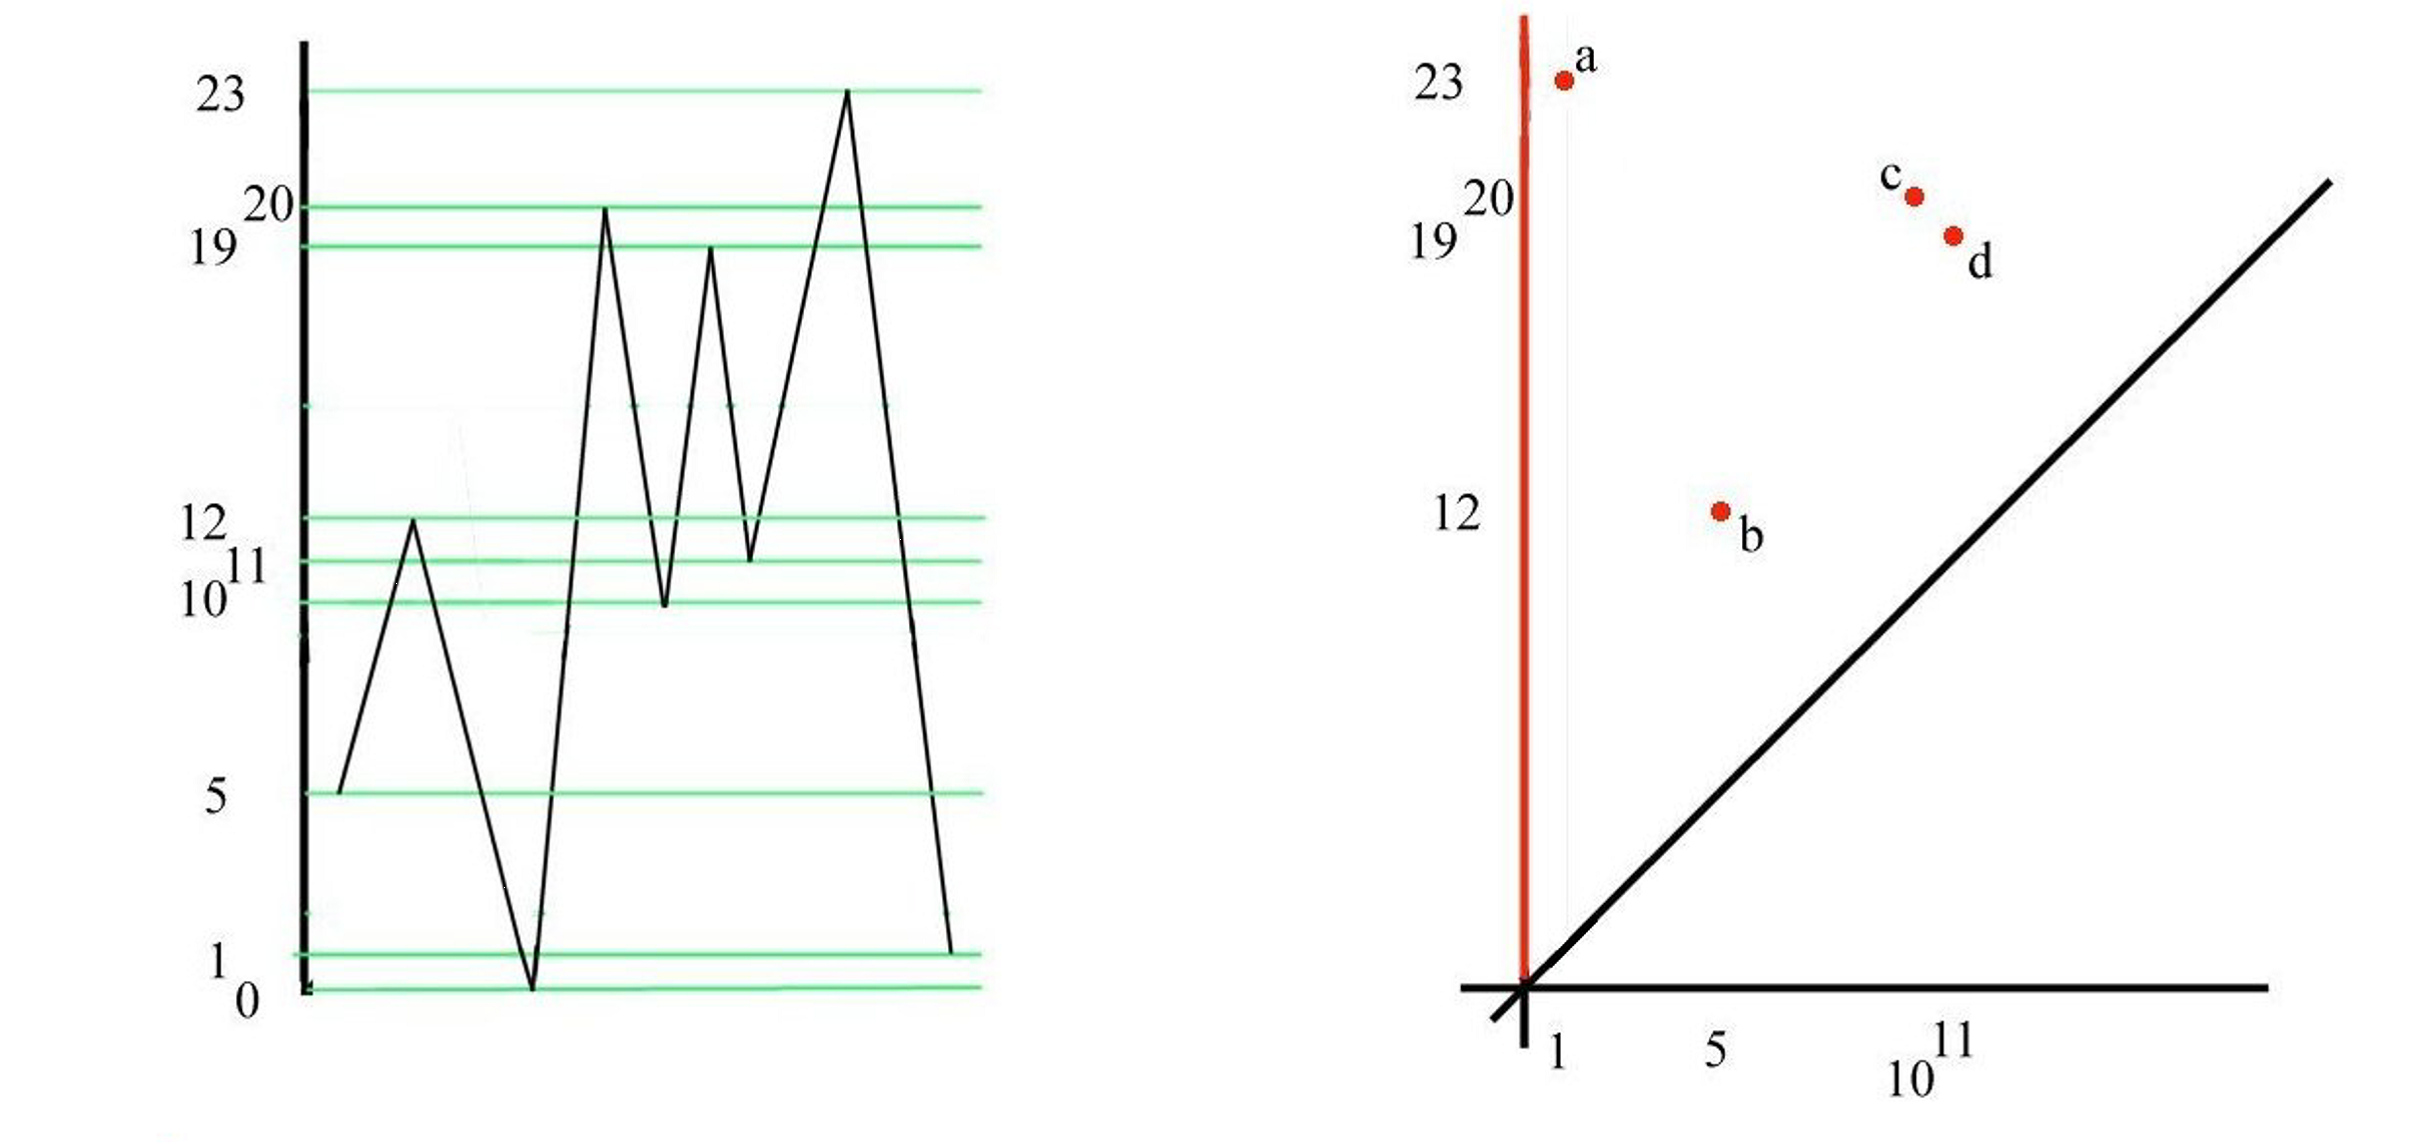
\includegraphics[height=7cm]{filtration example.png}
\caption{Figure borrowed from [Gur21]. Initial object (on the left) and the corresponding $0$-PD through the filtering function
"height" (right).}\label{fig:filtration example}
\end{figure}

\begin{figure}[tb]
\centering
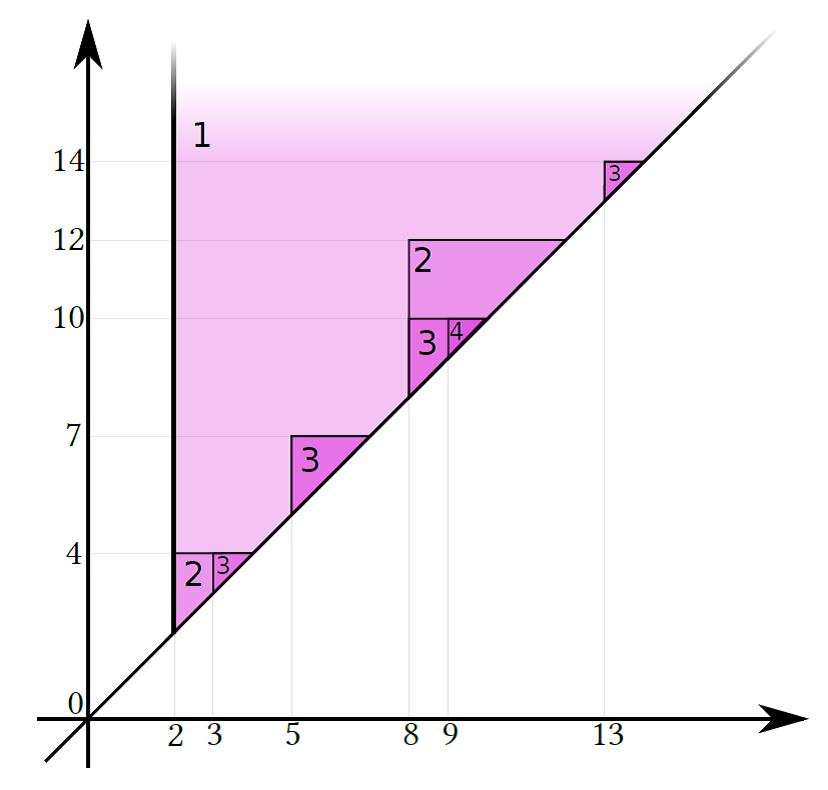
\includegraphics[height=7cm]{Ziggurat 2D.png}
\caption{Persistence Diagram $D$. Figure borrowed from [Gur21].}\label{fig:Ziggurat 2D}
\end{figure}

\begin{figure}[tb]
\centering
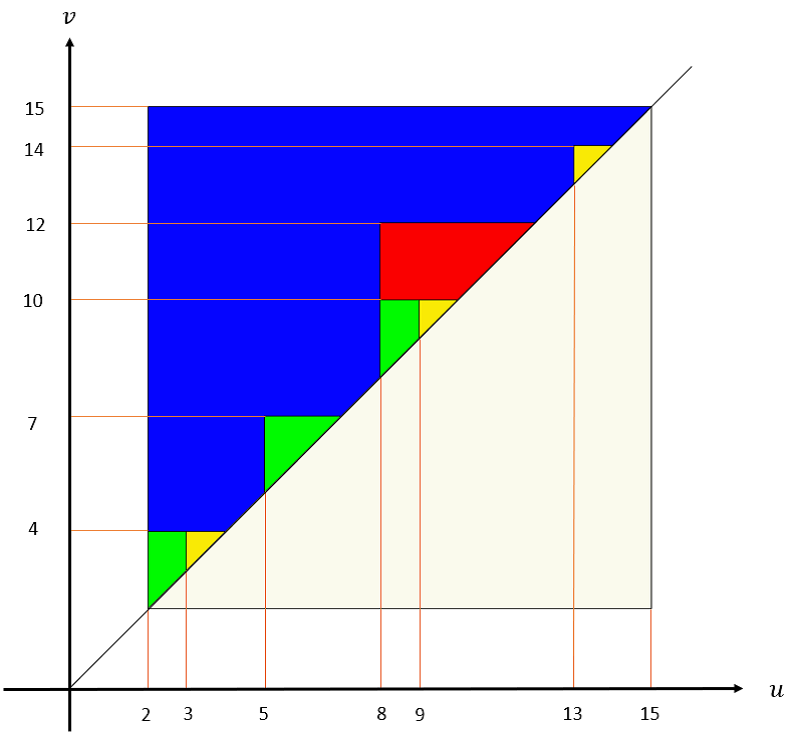
\includegraphics[height=7cm]{Ziggurat 1.png}
\caption{Figure borrowed from [Gur21]. View from top. In yellow, the prisms corresponding to cornerpoints with
persistence $1$, in green persistence those with $2$, in red those with persistence $4$, in blue the prism relative to the cornerpoint with the greatest persistence.
}\label{fig:Ziggurat 1}
\end{figure}

\begin{figure}[tb]
\centering
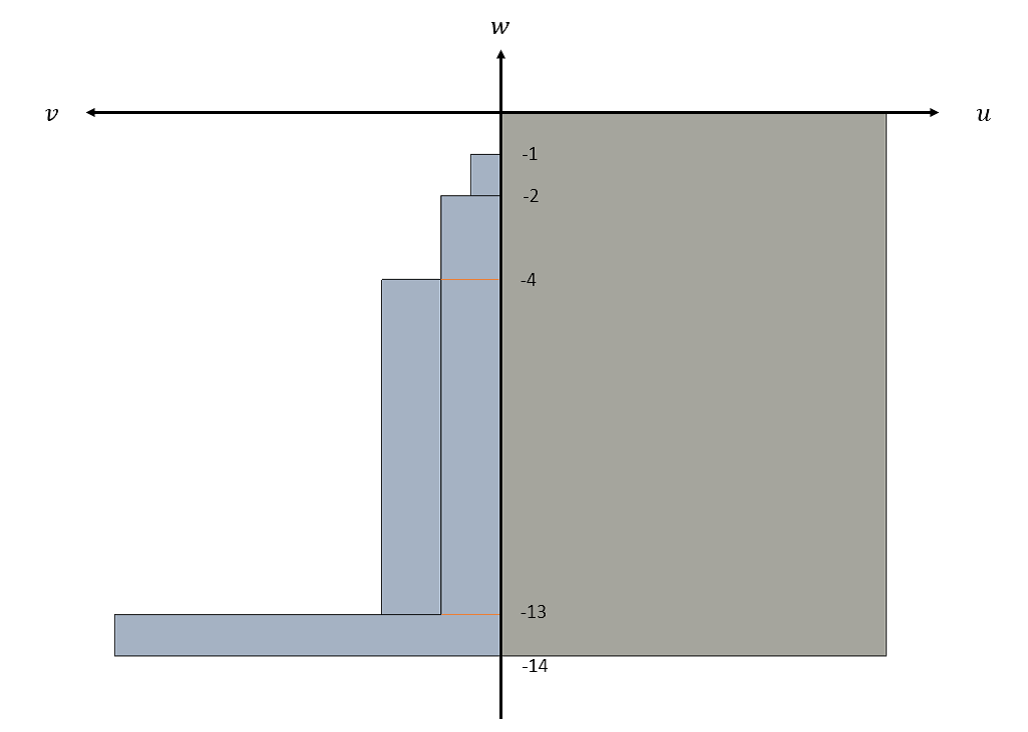
\includegraphics[height=7cm]{Ziggurat 2.png}
\caption{Figure borrowed from [Gur21]. Side view.}\label{fig:Ziggurat 2}
\end{figure}

\begin{figure}[tb]
\centering
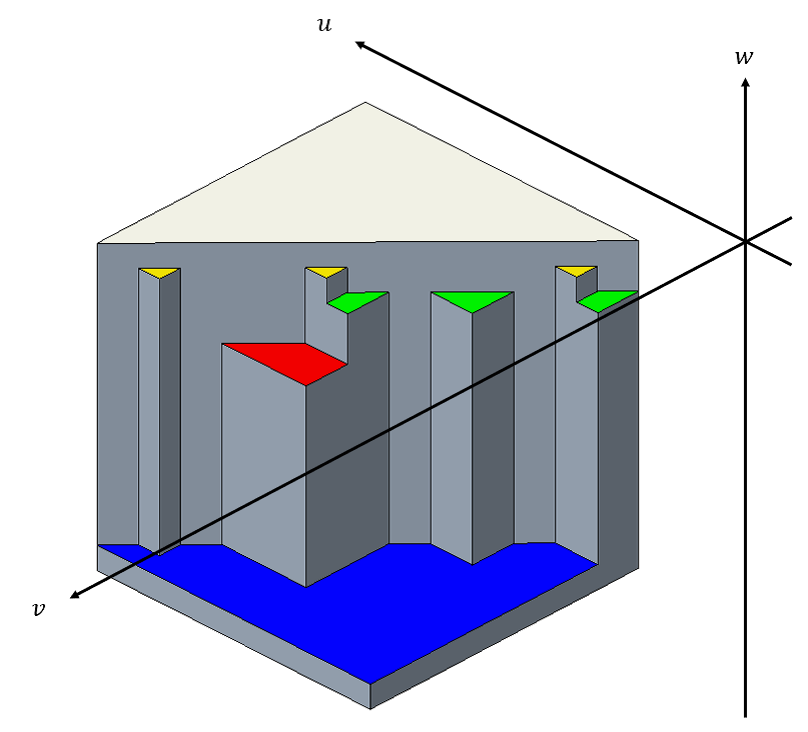
\includegraphics[height=10cm]{Ziggurat 3.png}
\caption{Figure borrowed from [Gur21]. Front view. }\label{fig:Ziggurat 3}
\end{figure}

\begin{figure}[tb]
\centering
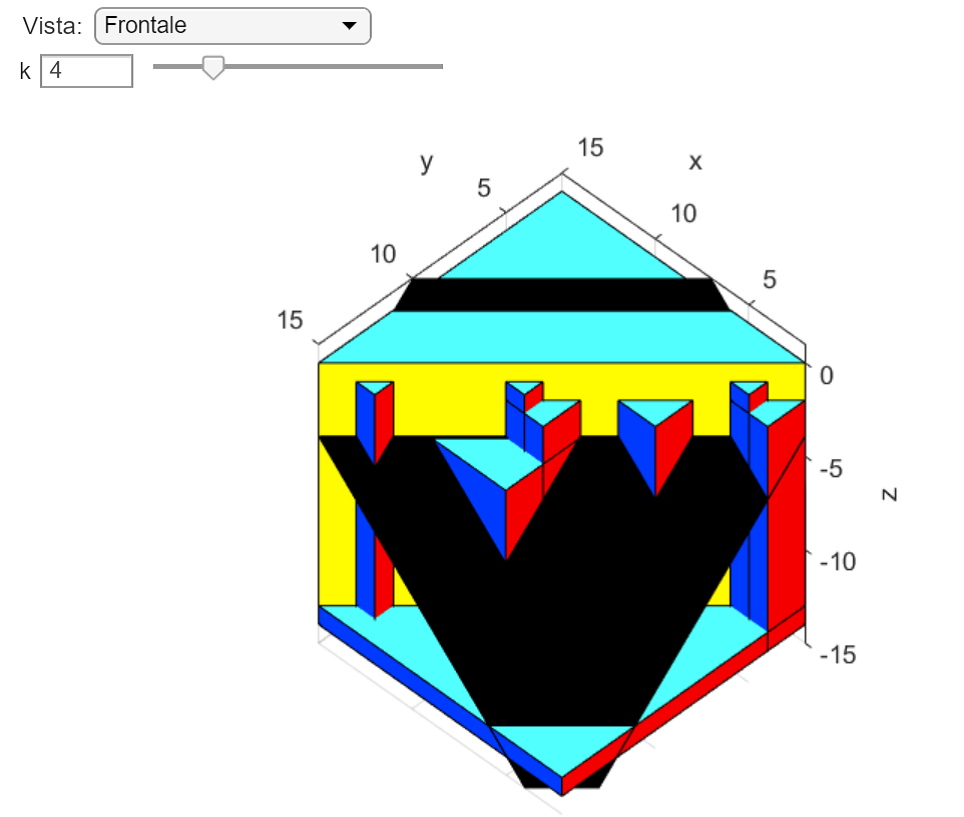
\includegraphics[height=10cm]{Ziggurat 3D.png}
\caption{Figure borrowed from [Gur21]. Frontal view of the Ziggurat cutted by the plane of equation $f_{Z_D}(u,v,w) = u-v-w = 4$.}\label{fig:Ziggurat 3D}
\end{figure}

\begin{figure}[tb]
\centering
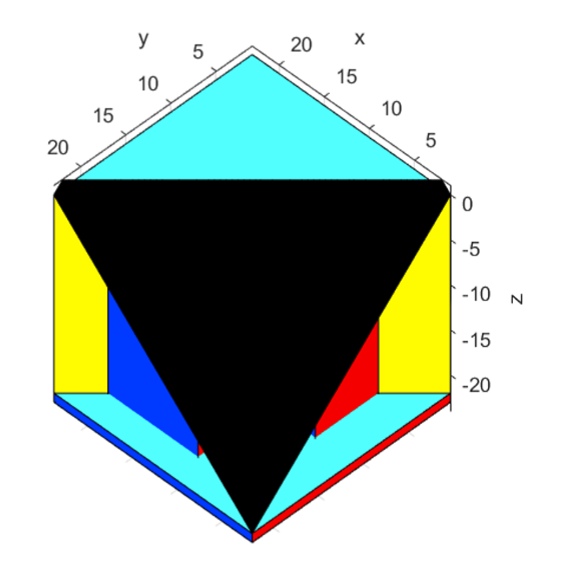
\includegraphics[height=10cm]{Ziggurat 3D k=0.png}
\caption{Figure borrowed from [Gur21]. Frontal view of the Ziggurat cutted by the plane of equation $f_{Z_D}(u,v,w) = u-v-w = 0$ ($k=0$).}\label{fig:Ziggurat 3D k=0}
\end{figure}

\begin{figure}[tb]
\centering
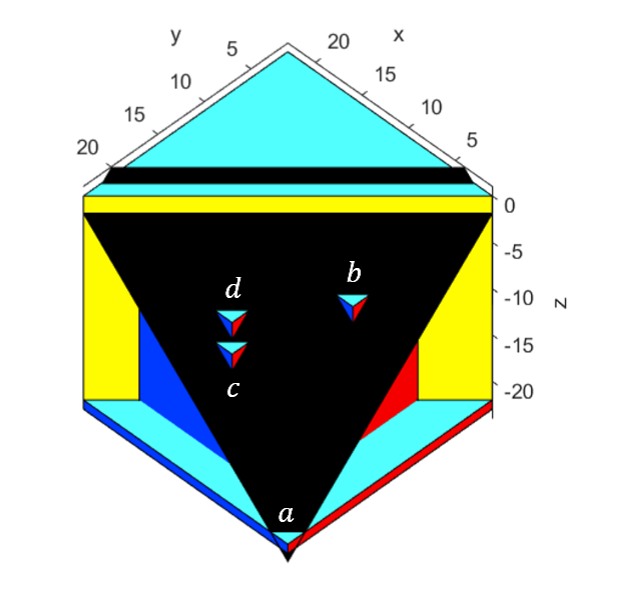
\includegraphics[height=10cm]{Ziggurat 3D k=2.png}
\caption{Figure borrowed from [Gur21]. Frontal view of the Ziggurat cutted by the plane of equation $f_{Z_D}(u,v,w) = u-v-w = 2$ ($k=2$).}\label{fig:Ziggurat 3D k=2}
\end{figure}

\begin{figure}[tb]
\centering
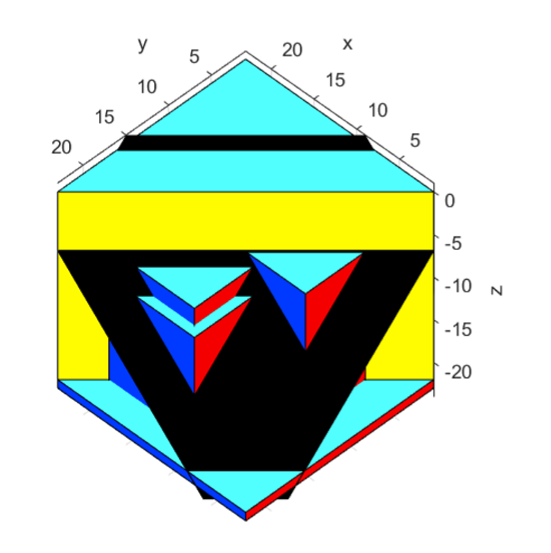
\includegraphics[height=10cm]{Ziggurat 3D k=7.png}
\caption{Figure borrowed from [Gur21]. Frontal view of the Ziggurat cutted by the plane of equation $f_{Z_D}(u,v,w) = u-v-w = 7$ ($k=7$).}\label{fig:Ziggurat 3D k=7}
\end{figure}

\begin{figure}[tb]
\centering
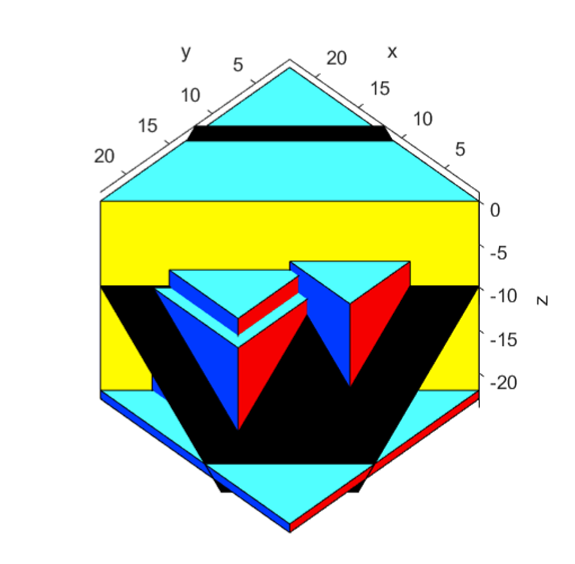
\includegraphics[height=10cm]{Ziggurat 3D k=10.png}
\caption{Figure borrowed from [Gur21]. Frontal view of the Ziggurat cutted by the plane of equation $f_{Z_D}(u,v,w) = u-v-w = 4$ ($k=4$).}\label{fig:Ziggurat 3D k=10}
\end{figure}

\begin{figure}[tb]
\centering
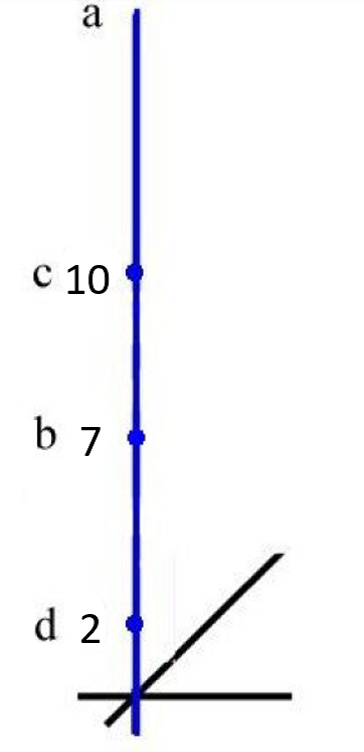
\includegraphics[height=10cm]{Ziggurat persistence diagram.png}
\caption{Figure borrowed from [Gur21]. $0$-persistence diagram of the pair $(Z_D, u-v-w)$
where $D$ refers to the diagram in figure~\ref{fig:filtration example}}\label{fig:Ziggurat persistence diagram}
\end{figure}

\begin{figure}[tb]
\centering
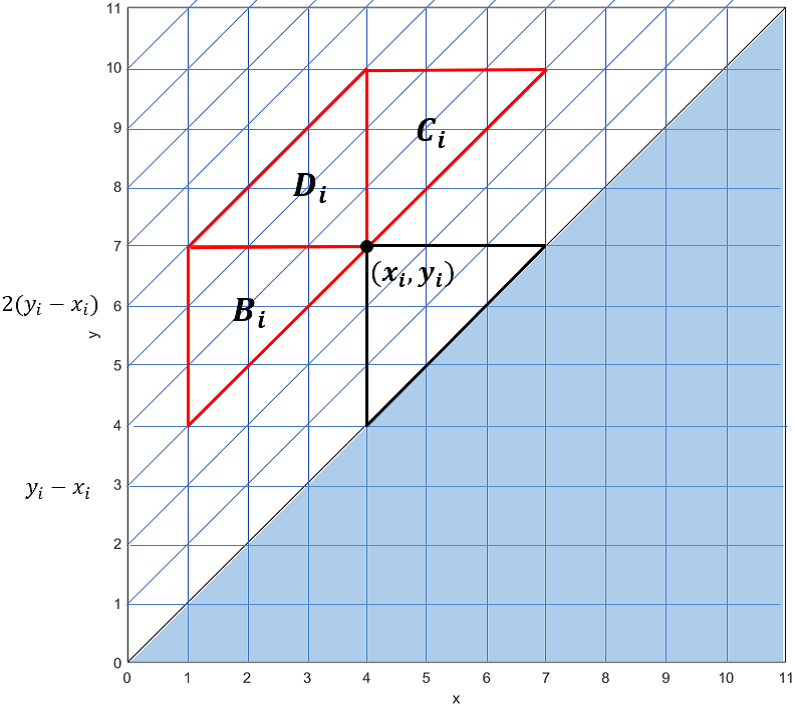
\includegraphics[height=10cm]{Ziggurat algorithm.png}
\caption{Figure borrowed from [Gur21]. Graphic display of the selection algorithm.}\label{fig:Ziggurat algorithm}
\end{figure}


\begin{figure}[tb]
\centering
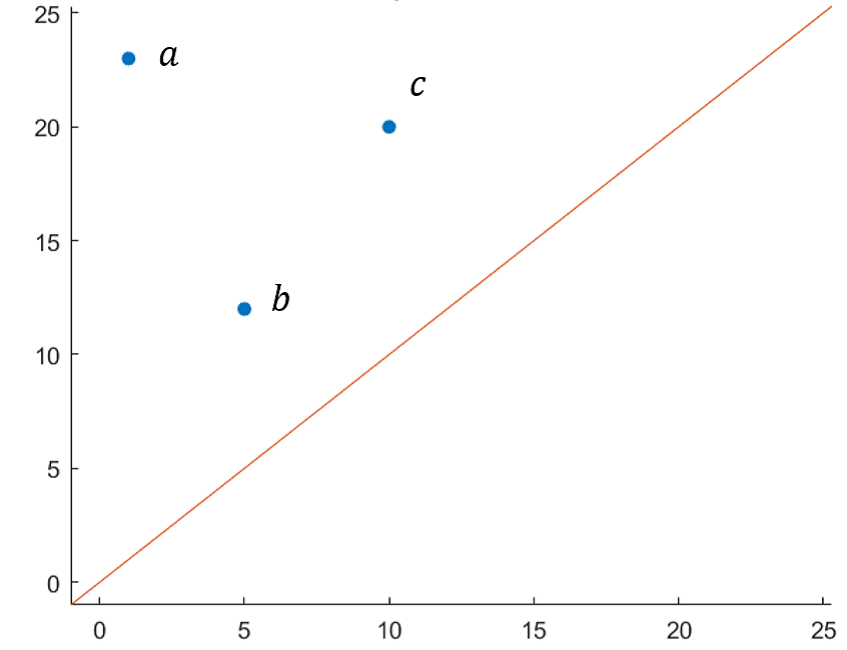
\includegraphics[height=10cm]{Kurlin selection.png}
\caption{Figure borrowed from [Gur21]. Selected cornerpoints with Kurlin's rule from the diagram on the left side of figure ~\ref{fig:filtration example}}\label{fig:Kurlin selection}
\end{figure}

\begin{figure}[tb]
\centering
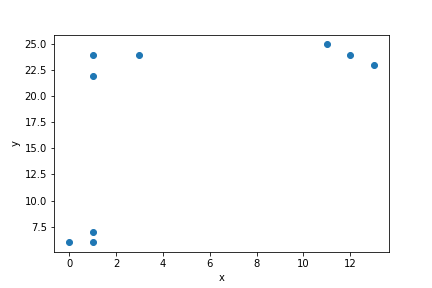
\includegraphics[height=7cm]{dgm_Massimo_repr.png}
\caption{Persistence diagram of the example~\ref{Example 2}}\label{fig:dgm_Massimo}
\end{figure}



\begin{figure}[!bth]
  \centering
		\subfigure[center][Persistence diagram of the Ziggurat of the diagram~\ref{fig:dgm_Massimo} colored according to cornerpoints' levels: a relevance ranking is provided for the original diagram.]{\label{fig:M8}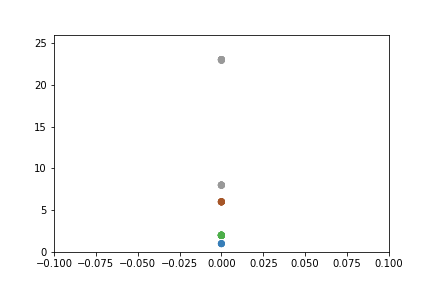
\includegraphics[width=0.45\textwidth]{M8.png}}
		\subfigure[center][Cornerpoints of the original persistence diagram~\ref{fig:dgm_Massimo} colored according to their levels.]{\label{fig:M2_8}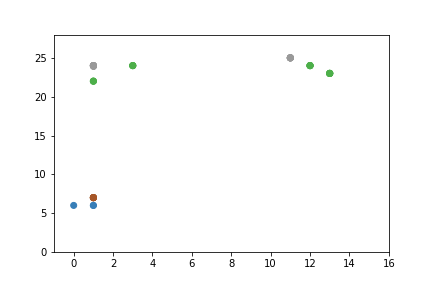
\includegraphics[width=0.45\textwidth]{M2_8.png}}
		\subfigure[center][Cornerpoints seletion with Kurlin's rule in the Ziggurat persistence's diagram. Cornerpoints above the widest gap are selected.]{\label{fig:M8}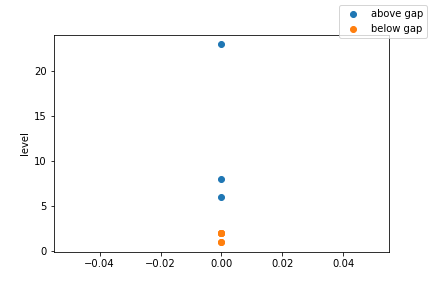
\includegraphics[width=0.45\textwidth]{plot_gap_1D.png}}
		\subfigure[center][According to Kurlin's rule, for each  ``cluster'' a cornerpoint is selected. ]{\label{fig:M2_8}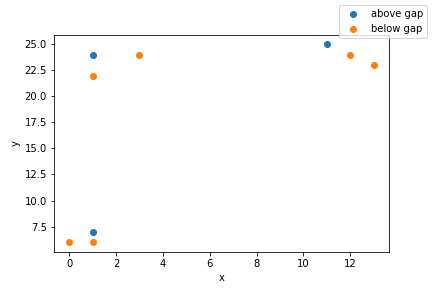
\includegraphics[width=0.45\textwidth]{plot_gap.png}}
  \caption{The correspondence of cornerpoints in the Ziggurat's persistence diagram with the respective ones in the starting diagram, distinguished by level (above) and by whether they are above or below the widest gap (below).}
  \label{fig:Label-figura-complessiva}
\end{figure}







\appendix

\chapter{Python Code for the persistence-image-based approach}
\label{appendix A}



\section{}

\chapter{Python Code for the Ziggurat}
\label{appendix B}








\printbibliography

\end{document}